\chapter{Verifying $N$-qubit GHZ States}
\label{chapter3}
%\\ via Multiple Quantum Coherences
%Until quantum error correction couldn't be implemented and fault-tolerant quantum computing still a rather distant dream, a new era in quantum technology is arising. Noisy Intermediate-Scale Quantum (NISQ) computers will be available in the next few years. Here “intermediate scale” refers to the size of quantum computers with a number of qubits ranging from 50 to a few hundred; that’s beyond what can be simulated by brute force using the most powerful existing digital supercomputers. \footnote{ For more details see \cite{PreskillNote}.}

In this chapter, we focus on the creation through a quantum circuit of a particular entangled state, the GHZ state, in order to test the IBM and Google quantum computers. 
Quantum computers are beset with a certain amount of noise, so we need to quantify the goodness of a prepared state respect to the state we want to create. 
This can be done through fidelity measurements, that measure the probability that the prepared state coincides with the state we want.

 First of all, we illustrate an experimental method to verify the generation of the GHZ state. It consists on measuring the multiple quantum coherences (MQC) \cite{Article} to infer the fidelity of the state we prepared. In fact, from MQC measurement it is possible to bound the state fidelity. The circuit implemented in this method is called MQC circuit.

Then such a MQC circuit of $N$-qubit is implemented in Qiskit software to be run on the IBM quantum computer; it is simulated on Qasm Simulator in ideal and noisy conditions. MQC measurements are done in both conditions. Afterwards the $N$-qubit circuit is executed on IBM Q Yorktown and IBM Q Melbourne, and we characterize the maximum number of $N$-qubit GHZ state that these devices support by MQC estimations.
After that, we focus on Cirq software. The MQC circuit is implemented for $N=5$ qubits and we add noise channels, as amplitude damping or depolarizing channels, to the circuit to study the fidelity bounds of the GHZ state in noisy conditions. Then, we build a circuit for creating a GHZ state of $N=5$ qubits and we add noise channels as previously. We measure the elements of the density matrix of the system. Finally, a circuit designed to create a \textit{Bell state}, is implemented, noise channels are added and we quantify the entanglement through concurrence measurements.



\section{Experimental method to measure MQC}
\label{theory}

The  \textit{ideal} GHZ state is illustrated in Eq. (\ref{15_firstchapter}).
It has amplified sensitivity  to phase rotations of each of the individual qubits in the entangled state. If each qubit has a phase rotation of $\phi$, then the $N$-qubit rotates collectively by $N\phi$. 
In presence of noise, the GHZ will be partially mixed and therefore a different phase may be observed; by observing how sensitive a \textit{non-ideal} GHZ state responds to phase rotations, it is possible to deduce how much entangled the state is. To this purpose, we need to measure multiple quantum coherence (MQC). The quantum circuit we use to prepare the GHZ state and measure MQC is shown in Figure \ref{MQCCircuit}. 
The collective rotation  applied on each qubit is given by the unitary operator $ U_{\phi} = e^{-i \frac{\phi}{2}\sum_j \sigma_{z}^{j}}$.

\begin{center}

\[ 
\Qcircuit @C=1.2em @R=0.7em {
\lstick{\ket{0}} & \gate{H} & \multigate{3}{U_{CX}} &  \gate{U_{\phi}}& \multigate{3}{U_{CX}^{\dagger}} & \gate{H}  & \meter \\
 \lstick{\ket{0}} & \qw & \ghost{U_{CX}}  & \gate{U_{\phi}} & \ghost{U_{CX}^{\dagger}} & \qw &  \meter \\
 \lstick{ \vdots \ }& \qw & \ghost{U_{CX}} & \gate{U_{\phi}} & \ghost{U_{CX}^{\dagger}} & \qw  &  \meter \\
 \lstick{\ket{0}}& \qw &  \ghost{U_{CX}} &  \gate{U_{\phi}} & \ghost{U_{CX}^{\dagger}} &\qw & \meter
}
 \]
 
 \captionof{figure}{MQC quantum circuit for $N$ qubits.}
\label{MQCCircuit}

\end{center}

\noindent The quantum circuit for measuring MQC can be described in four steps \cite{Article}:



%\begin{center}
%
%\[ 
%\Qcircuit @C=1em @R=1em {
%\lstick{\ket{0}} & \gate{H} & \multigate{3}{U_{CX}} &  \multigate{3}{\text{Sensing}}& \multigate{3}{U_{CX}^{\dagger}} & \gate{H}  & \meter \\
% \lstick{\ket{0}} & \qw & \ghost{U_{CX}}  & \ghost{\text{Sensing}} & \ghost{U_{CX}^{\dagger}} & \qw &  \qw \\
% \lstick{ \vdots \ }& \qw & \ghost{U_{CX}} &  \ghost{\text{Sensing}} & \ghost{U_{CX}^{\dagger}} & \qw  &  \qw \\
% \lstick{\ket{0}}& \qw &  \ghost{U_{CX}} &  \ghost{\text{Sensing}} & \ghost{U_{CX}^{\dagger}} &\qw & \qw
%}
% \]
% 
% \captionof{figure}{Quantum sensing circuit.}
%\label{QuantumSensingCircuit}
%
%\end{center}

\begin{enumerate}

\item Starting from the $N$-qubit ground state: $\ket{\text{GS}} = \ket{000 \dots 0}$, apply a Hadamard gate on qubit 0 followed by a sequence of CX gates. Ideally this brings the system into the GHZ state: $\ket{\text{GHZ}}= \frac{1}{\sqrt{2}}(\ket{000 \dots 0} + \ket{111 \dots 1})$.

\item Apply a collective rotation given by the unitary $U_{\phi}$ on all qubits. This amounts to adding a phase $N \phi$ to the GHZ state: $\ket{\text{GHZ}}= \frac{1}{\sqrt{2}}(\ket{000 \dots 0} + e^{-i N \phi} \ket{111 \dots 1})$.

\item Disentangle the GHZ state by performing the CX gate sequence in reverse order. The amplified phase is mapped onto qubit 0: $\frac{1}{\sqrt{2}}(\ket{0}+e^{-i N \phi} \ket{1}) \otimes  \ket{00 \dots 0}$. Finally, apply a Hadamard gate on qubit 0: $(\cos{\frac{N \phi}{2}}\ket{0}+i \sin{\frac{N \phi}{2}} \ket{1}) \otimes  \ket{00 \dots 0}$.

\item Read out the amplified phase by measuring the probability of the system returning to its initial state: $\ket{\text{GS}}$. Therefore, a measurement gate on each qubit it is applied.
\end{enumerate}


\vspace{0.3cm}
\noindent Now, define $U_{GHZ}=U_{CX}H_0$, where $H_0$ refers to Hadamard gate applied on qubit 0. The measured signal is given by:

\begin{equation}
 S_{\phi} = \abs{\bra{000 \dots 0} U_{GHZ}^{\dagger} U_{\phi} U_{GHZ} \ket{000 \dots 0} }^2  = \tr (\rho_\phi \rho) 
 \label{S_phi} 
\end{equation}

\noindent where $\rho = U_{GHZ} \ket{000 \dots 0} \bra{000 \dots 0} U_{GHZ}^{\dagger}$ and $\rho_\phi = U_\phi \rho U_\phi^\dagger$. 
 In the ideal case, if there is no decoherence Eq. (\ref{S_phi}) reduces to

\begin{equation}
 S_{\phi}^{\text{ideal}} = \frac{1}{2} (1 + \cos{N \phi}) 
 \label{S_phi_ideal}
 \end{equation}

\noindent Any difference between the measured $S_{\phi}$ and $S_{\phi}^{\text{ideal}}$ is an indication that the GHZ state is imperfect. The parameter is $\phi = \frac{ \pi j }{N+1}$, where $j=0,1,2,\dots,2N+1$. 

The \textbf{MQC amplitudes} are defined as the discrete Fourier transform of $S_{\phi}$:

\begin{equation}
I_{q}= \mathcal{N}^{-1} | \sum_{\phi} e^{i q \phi} S_{\phi} | 
\label{I_q}
\end{equation} 

\noindent where $\mathcal{N} = 2(N+1)$ is a normalization factor. Let us note that they are symmetric: 

\begin{equation}
I_q=I_{-q}.
\label{I_q_2}
\end{equation} 

\noindent For an ideal $N$-qubit GHZ state , the nonzero elements in the density matrix resides only in the four corners. Therefore only three components arise in the expansion:
$\rho^{GHZ} = \rho_0^{GHZ} + \rho_N^{GHZ} + \rho_{-N}^{GHZ}$. Explicitly they are given by

\begin{equation}
   \begin{gathered}
 \rho_0^{GHZ}  = \frac{1}{2} ( \ket{000\dots0}\bra{000\dots0} + \ket{111\dots1}\bra{111\dots1})  \\
\rho_N^{GHZ}  = \frac{1}{2} \ket{000\dots0}\bra{111\dots1}  \\
 \rho_{-N}^{GHZ} = \rho_N^{GHZ^{\dagger}} 
	\end{gathered}
\end{equation} 

\noindent The corresponding multiple quantum amplitudes are 

%\begin{equation}
%I_0^{GHZ} = \tr (\rho_0^{GHZ} \rho_0^{GHZ}) = \frac{1}{2}, \quad I_N^{GHZ} = \tr (\rho_N^{GHZ} \rho_{-N}^{GHZ}) = \frac{1}{4}, \quad  I_{-N}^{GHZ} =  I_N^{GHZ}
%\end{equation} 

\begin{equation}
I_0^{GHZ} = \frac{1}{2}, \quad I_N^{GHZ} = \frac{1}{4}, \quad  I_{-N}^{GHZ} =  I_N^{GHZ}
\end{equation} 


\noindent The $I_q$ are used to quantify the state fidelity. The $N$-qubit GHZ state fidelity defined as $ F= \bra{GHZ} \rho \ket{GHZ} $ can be bounded by \footnote{The proof can be found in the supplementary material section of \cite{Article}.}:

\begin{equation}
 2 \sqrt{I_N} \leq F \leq \sqrt{I_0/2} + \sqrt{I_N}.
 \label{Fidelity_Bounded}
 \end{equation}

\noindent For a perfect GHZ state F=1: $I_0=2 I_N=1/2$ and all other $I_q$ being zero. 
For a $N$-qubit state to have multipartite GHZ entanglement, it needs to have a minimal fidelity of 0.5 \cite{Fidelity}. 

%It has been experimented that adding a $\pi$-pulse after making the GHZ state can dramatically improve the measured fidelity. Therefore a quantum X gate is applied on all qubits before $U_{\phi}$ as shown in Figure \ref{MQCCircuitX}.
%
%\begin{center}
%
%\[ 
%\Qcircuit @C=1em @R=1em {
%\lstick{\ket{0}} & \gate{H} & \multigate{3}{U_{CX}} &  \gate{X} & \gate{U_{\phi}}& \multigate{3}{U_{CX}^{\dagger}} & \gate{H}  & \meter \\
% \lstick{\ket{0}} & \qw & \ghost{U_{CX}}  & \gate{X} & \gate{U_{\phi}} & \ghost{U_{CX}^{\dagger}} & \qw &  \meter \\
% \lstick{ \vdots \ }& \qw & \ghost{U_{CX}} & \gate{X} & \gate{U_{\phi}} & \ghost{U_{CX}^{\dagger}} & \qw  &  \meter \\
% \lstick{\ket{0}}& \qw &  \ghost{U_{CX}} & \gate{X} & \gate{U_{\phi}} & \ghost{U_{CX}^{\dagger}} &\qw & \meter
%}
% \]
% 
% \captionof{figure}{Refocused MQC quantum circuit.}
%\label{MQCCircuitX}
%\end{center}

\section{MQC Circuit on Qiskit software}
\label{Qiskitsection}

Following the protocol given in the previous section, we realize the experimental quantum circuit for measuring MQC, called MQC circuit, for different values of $N$ qubits and we execute it on different backends provided by IBM. 
The experimental matrix $U_{\phi}$ implemented in the circuit has the following form: 

\begin{equation}
U_{\phi} =  \begin{pmatrix} e^{- i \frac{\phi}{2} } & 0 \\ 0 & e^{ i \frac{\phi}{2} } \end{pmatrix}  
\label{U_gate_MQC}
\end{equation}

\subsection{Measurements and analysis}
\label{analysis}

\noindent For each value of $N$ and regardless of the backend used, it is possible to describe generally how the results are obtained and analyzed:
\begin{enumerate}
	\item The value of $\phi $ is fixed; the backend executes the quantum circuits $k$ times and returns a count dictionary containing the final values of any classical registers in the circuit.
	\item The count of the state  $\ket{000\dots0}$ is taken because it correspond with the measurement $S_{\phi}$ in Eq. (\ref{S_phi}). Then that count is divided by $k$ to obtain it in the range from 0 to 1.
	\item The first two steps are executed again for each value of $\phi = \frac{ \pi j }{N+1}$, where $j=0,1,2,\dots,2N+1$. In that way, a list of counts at different values of $\phi$ is obtained.
	\item A plot of the function $S_{\phi}^{\text{ideal}}$ in Eq. (\ref{S_phi_ideal}) is done; it represents the theoretical results the experiment should give. Then the experimental list of data is plotted in function of $\phi$ and it is compared with such a theoretical plot.
	\item The MQC amplitudes are calculated by the discrete Fourier transform $I_q$,  in Eq. (\ref{I_q}), of that list and plotted in the range $[-N,N]$. They are compared with the MQC amplitudes obtained by the Fourier transform of $S_{\phi}^{\text{ideal}}$. Then, the fidelity can be bounded as in Eq. (\ref{Fidelity_Bounded}).
\end{enumerate}

%The experimental data are analyzed in the following way.
%\begin{enumerate}
%	\item Firstly, a plot of the function $S_{\phi}^{\text{ideal}}$ (equation \ref{S_phi_ideal}) is done. It represents the theoretical results the experiment should give.
%	\item The experimental list of data, obtained by the previous procedure, is plotted in function of $\phi$. 
%	\item The MQC amplitudes are calculated by the discrete Fourier transform $I_q$  of that list as in the equation \ref{I_q} and plotted. Then, the fidelity can be bounded as in \ref{Fidelity_Bounded}.
%\end{enumerate}

\subsection{Simulation}
The $N$-qubit MQC circuit is executed on Qasm Simulator of IBM. Firstly, we suppose an execution of the circuit in an ideal condition, then we consider a noise model based upon the real quantum device IBM Q Melbourne.

\subsubsection{Ideal model}

Consider an ideal execution, where the quantum circuit is supposed to be run on an ideal quantum device. The backend Qasm Simulator executes the circuit $k=8192$ times and returns a list of counts of the state  $\ket{000\dots0}$ for different $\phi$, as described in Section \ref{analysis}. 
The circuit is implemented and ideally simulated from $N=2,\dots,24$ qubits, until computational resources are enough to execute the circuit \footnote{The computational resources refers to a classical computer of 8 Gbyte of RAM.}.
The results obtained are very close to the theoretical expectation up to a statistical fluctuations given by the probabilistic simulation. For each $N$ the fidelity bounds, defined by Eq. (\ref{Fidelity_Bounded}), are $\sim 1$.  

For instance, we suppose $N=6$ qubits. The corresponding MQC circuit implemented in Qiskit is shown in Figure \ref{MQCCircuit6} and the ideal execution results are plotted in Figure \ref{IdealSimulation6}.   
In the plot on the left we compare the theoretical results $S_\phi$(line in red) to the experimental counts of the simulation (points in blue). The right plot shows the Fourier transform of $S_\phi^{\text{ideal}}$ (line in red) and the MQC amplitudes (\ref{I_q}) in such an ideal case for $N=6$ qubit (points in blue). The plots for all the other values of $N$ we have simulated  are similar and the fidelity is still good: for example, the results for $N=22$ qubit are shown in Figure \ref{IdealSimulation6}.



\begin{center}

\[ 
\Qcircuit @C=0.8em @R=1.1em {
\lstick{\ket{0}_0}	& \gate{H} & \ctrl{1}	 & \qw  &	 \qw & \qw	 & 	\qw  & \gate{U_{\phi}} 	& \qw & \qw & \qw & \qw & \ctrl{1} &  \gate{H}  &\meter \\
\lstick{\ket{0}_1}	& \qw	 & \targ  	&  \ctrl{1} 		      & \qw 	& \qw	& \qw &  \gate{U_{\phi}}	 &   \qw & \qw & \qw & \ctrl{1} & \targ & \qw &  \meter \\
\lstick{\ket{0}_2}	& \qw	 & \qw  	&  \targ 		      & \ctrl{1} & \qw 	& \qw & \gate{U_{\phi}}	 &   \qw & \qw & \ctrl{1} & \targ & \qw & \qw & \meter \\
\lstick{\ket{0}_3}	& \qw	 & \qw  	&  \qw 		      &  \targ &  \ctrl{1} & \qw &	\gate{U_{\phi}}	 &  \qw & 	\ctrl{1}  & \targ & \qw & \qw & \qw & \meter \\
\lstick{\ket{0}_4}	& \qw	 & \qw  	&  \qw 		      &  \qw  & \targ	& \ctrl{1} & \gate{U_{\phi}}	 &  \ctrl{1} & \targ &  \qw & \qw & \qw &  \qw & \meter \\
\lstick{\ket{0}_5}	& \qw	 & \qw  	&  \qw 		      &  \qw  & \qw	& \targ & \gate{U_{\phi}}	 &  \targ & \qw & \qw & \qw & \qw & \qw &  \meter \\
}
 \]
 
 \captionof{figure}{ MQC quantum circuit for $N = 6$ qubits.}
\label{MQCCircuit6}

\end{center}

\vspace{0.3cm}

\begin{figure}[h!]
\begin{minipage}[c]{0.5\linewidth}
\hspace{1cm}
\centering 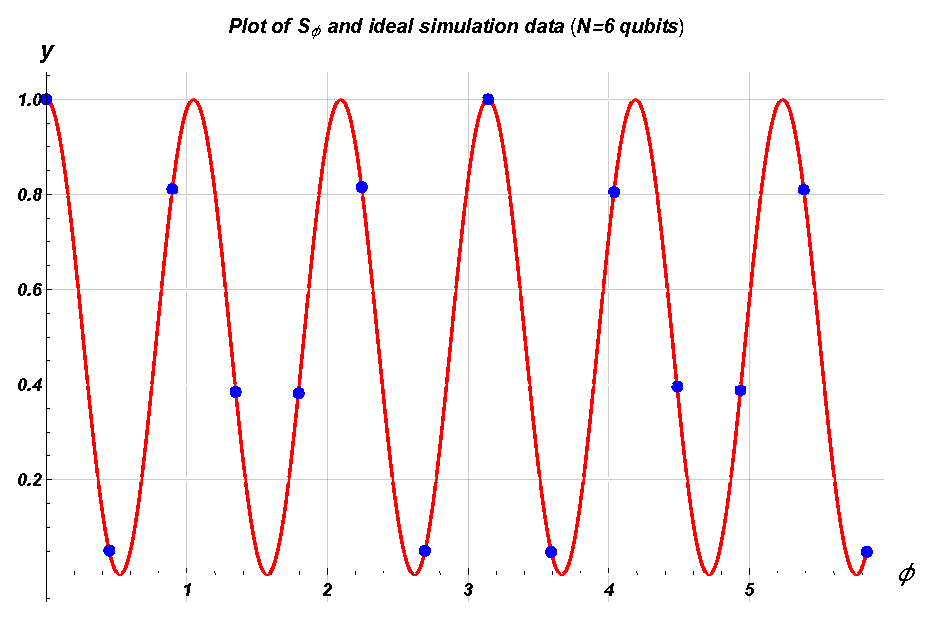
\includegraphics[width=1\textwidth]{./chapter3/graphics_IBM/simulation/6S.eps}
\end{minipage}
%\hspace{1mm}
\begin{minipage}[]{0.5\linewidth}
\centering 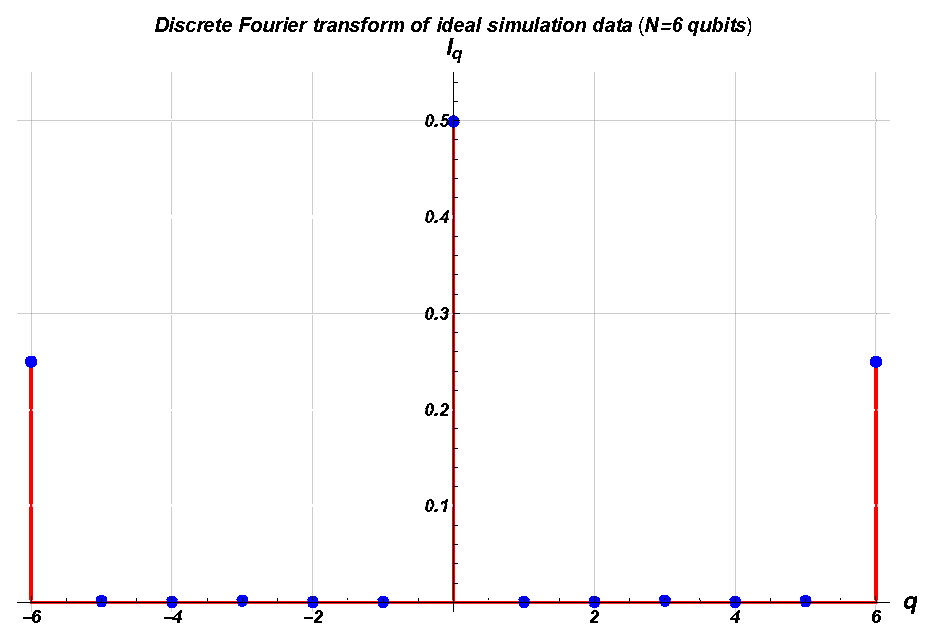
\includegraphics[width=1\textwidth]{./chapter3/graphics_IBM/simulation/6I.eps}
\end{minipage}
\caption{\label{IdealSimulation6} \textbf{N=6} qubits. Left:  plot of $S_{\phi}^{\text{ideal}}$ is represented in red, experimental measurements $S_{\phi}$ obtained by the simulation in the \textbf{Qasm Simulator} backend in the ideal case are drawn in blue. Right: corresponding MQC amplitudes $I_q$ of $S_\phi^{\text{ideal}}$ and $S_\phi$, respectively in red and blue.}
\end{figure}

\begin{figure}[h!]
\begin{minipage}[c]{0.5\linewidth}
\hspace{1cm}
\centering 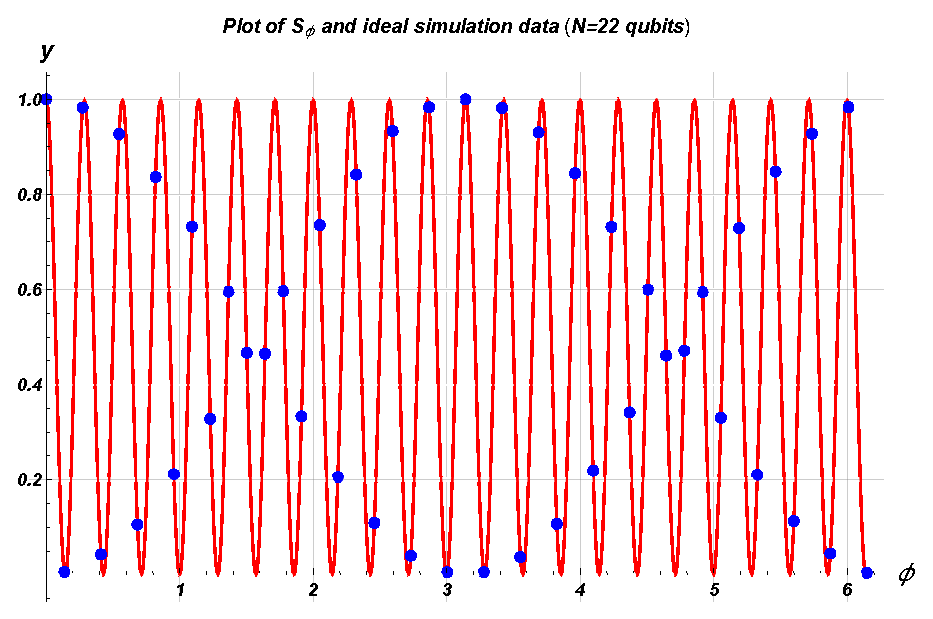
\includegraphics[width=1\textwidth]{./chapter3/graphics_IBM/simulation/22S.eps}
\end{minipage}
%\hspace{1mm}
\begin{minipage}[]{0.5\linewidth}
\centering 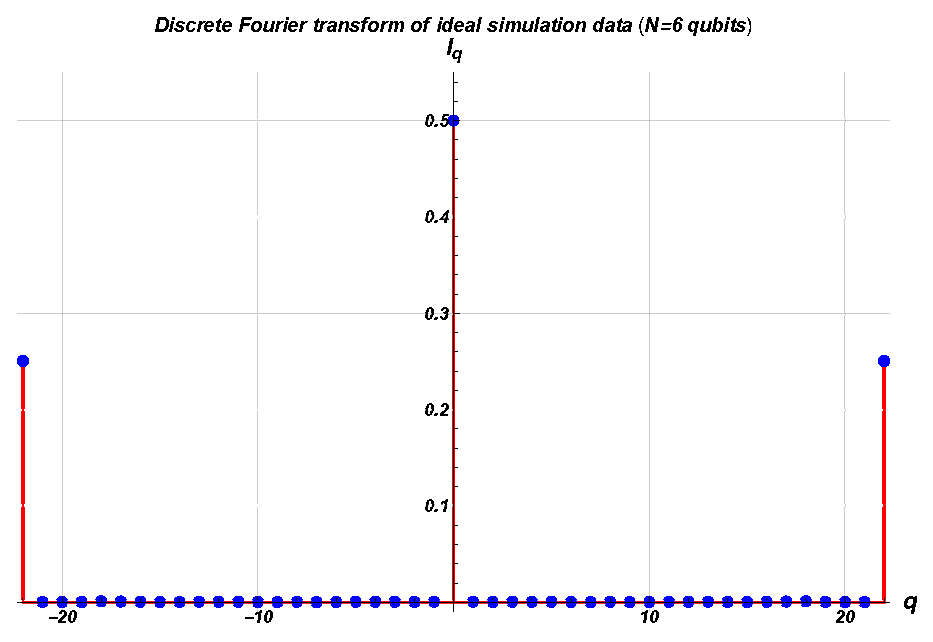
\includegraphics[width=1\textwidth]{./chapter3/graphics_IBM/simulation/22I.eps}
\end{minipage}
\caption{\label{IdealSimulation6}\textbf{N=22} qubits. Left:  plot of $S_{\phi}^{\text{ideal}}$ is represented in red, experimental measurements $S_{\phi}$ obtained by the simulation in the \textbf{Qasm Simulator} backend in the ideal case are drawn in blue. Right: corresponding MQC amplitudes $I_q$ of $S_\phi^{\text{ideal}}$ and $S_\phi$, respectively in red and blue.}
\end{figure}

\subsubsection{Noise model}

We apply the same protocol to a circuit implemented with a noise model associated to the IBM Q Melbourne device. Noise is added on all qubits and on all basis gates of this device. The read-out error is also implemented. These error values are available online \cite{TutorialQiskit}. In addiction, the typical gate time are provided. 
Since the IBM documentation does not currently provide the gate times for gates of this device we manually insert them, basing on values found online. 
The code used for doing the model is shown in Figure \ref{NoiseModel_code}. 

The circuit is simulated for $N=2,\dots,9$ qubits. For each value of $N$ the fidelity bounds are estimated as previously by measuring MQC obtained by discrete Fourier transform of $S_\phi$. 
We plot the fidelity lower and upper bounds in function of the number $N$ of qubits in Figure \ref{F_NoiseModel_ibmq16melbourne}. They are respectively the green and the orange points.
If the fidelity bounds are in the range $[0.5,1]$, we consider the GHZ state verified, as we mentioned in Section \ref{theory}. Otherwise, the fidelity level is not acceptable and the device is not able to create the GHZ state with a good confidence. In the case we are considering, the device is able to create a good GHZ state until $N=7$ qubit.
In Figure \ref{NoiseSimulation7}, we show the plots of $S_\phi$ and of $I_q$ for  $N=7$ qubits .



\begin{figure}[h!]

\begin{lstlisting}[language=Python]%[language=Python, caption=Python example]

device = IBMQ.get_backend('ibmq_16_melbourne')
properties = device.properties()
gate_times = [
    ('u1', None, 0), ('u2', None, 100), ('u3', None, 200),
    ('cx', [1, 0], 678), ('cx', [1, 2], 547), ('cx', [2, 3], 721),
    ('cx', [4, 3], 733), ('cx', [4, 10], 721), ('cx', [5, 4], 800),
    ('cx', [5, 6], 800), ('cx', [5, 9], 895), ('cx', [6, 8], 895),
    ('cx', [7, 8], 640), ('cx', [9, 8], 895), ('cx', [9, 10], 800),
    ('cx', [11, 10], 721), ('cx', [11, 3], 634), ('cx', [12, 2], 773),
    ('cx', [13, 1], 2286), ('cx', [13, 12], 1504), ('cx', [], 800)]

# Construct the noise model from backend properties and custom gate times
noise_model = noise.device.basic_device_noise_model(properties, gate_times=gate_times)
print(noise_model)
 
\end{lstlisting}

\caption{\label{NoiseModel_code} Python code on Qiskit for building the device noise model based upon 'ibmq melbourne' real quantum device. The gate times are taken from \cite{TutorialQiskit}.}
\end{figure}

\vspace{0.3cm}

\begin{figure}[h!]
\begin{minipage}[c]{0.5\linewidth}
\hspace{1cm}
\centering 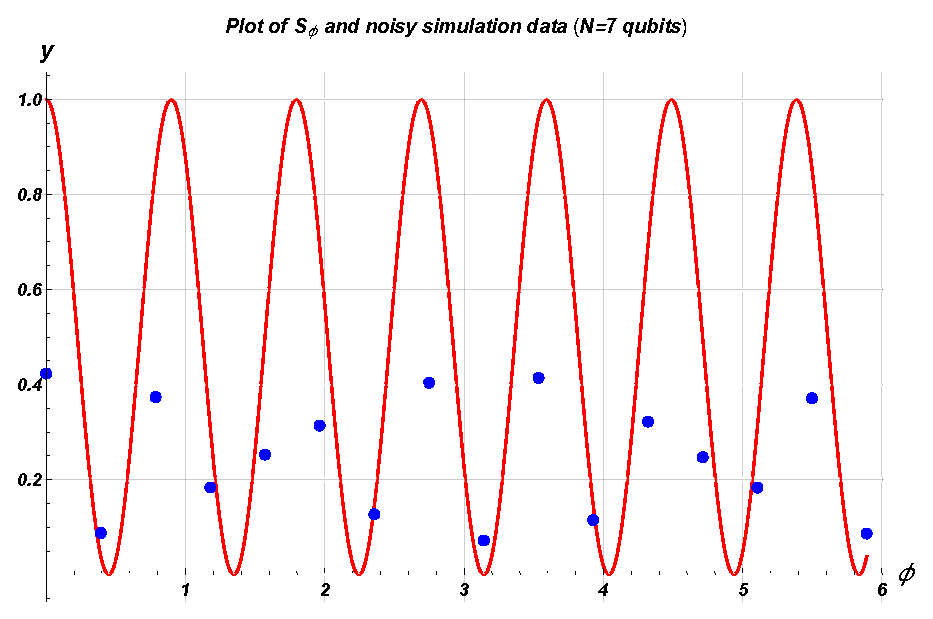
\includegraphics[width=1\textwidth]{./chapter3/graphics_IBM/simulation/7S_noise.eps}
\end{minipage}
%\hspace{1mm}
\begin{minipage}[]{0.5\linewidth}
\centering 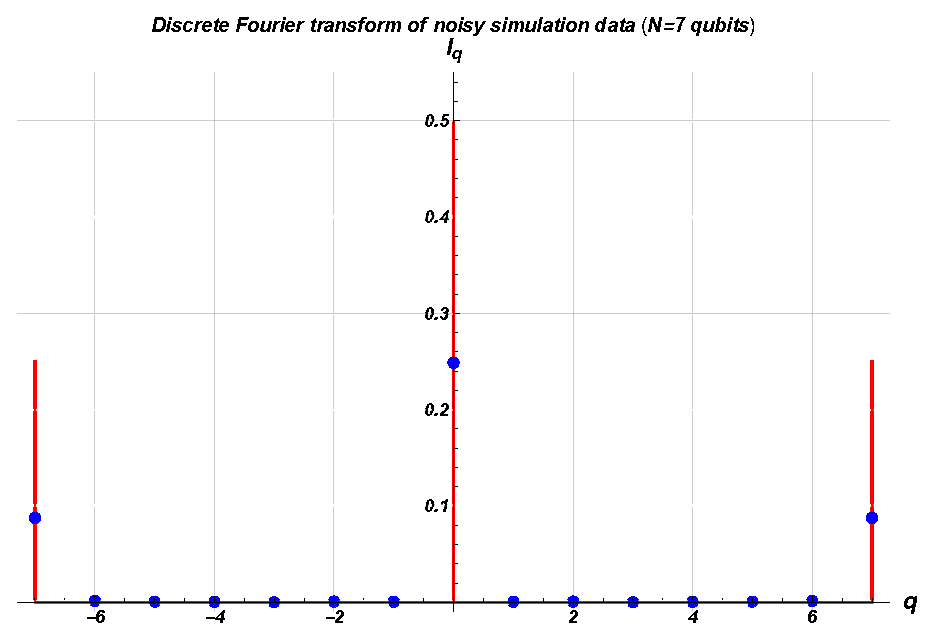
\includegraphics[width=1\textwidth]{./chapter3/graphics_IBM/simulation/7I_noise.eps}
\end{minipage}
\caption{\label{NoiseSimulation7} \textbf{N=7} qubits. Left:  plot of $S_{\phi}^{\text{ideal}}$ is represented in red, experimental measurements $S_{\phi}$ obtained by the simulation in the \textbf{Qasm Simulator} backend in noisy conditions are drawn in blue. Right: corresponding MQC amplitudes $I_q$ of $S_\phi^{\text{ideal}}$ and $S_\phi$, respectively in red and blue.}
\end{figure}


\begin{figure}[h!]
\centering 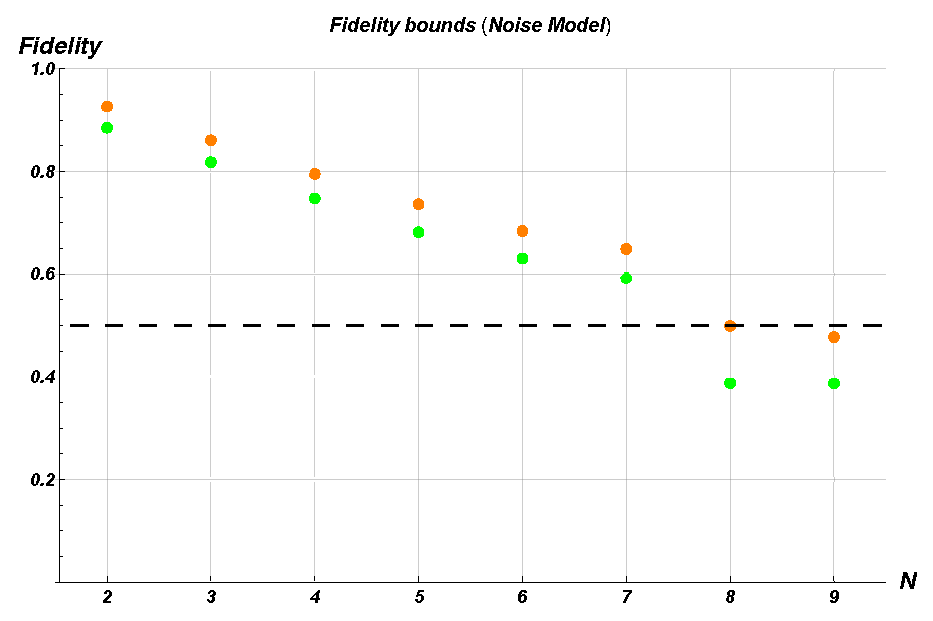
\includegraphics[width=0.7\textwidth]{./chapter3/graphics_IBM/simulation/NoiseModel_ibmq16melbourne.eps}
\caption{\label{F_NoiseModel_ibmq16melbourne} Fidelity lower bounds and upper bounds, respectively in green and orange, for the $N$-qubit MQC circuit, executed in a user-built \textbf{noisy device}, are plotted in function of the number of qubits $N$. The line dashed in black represents the limit of 0.5 and under that we consider the fidelity of the state not acceptable. }
\end{figure}


\newpage
\subsection{Run on real devices}

The MQC circuit is executed in two backends: IBM Q Yorktown and IBM Q Melbourne devices. For each device, we implement the circuit in two different ways:
\begin{enumerate}
\item In the first case, we add the gates in the MQC circuit taking no care on how the real hardware is built. It means that we always use the physical qubits from 0 to $N$, in order, of each device and that a sequence of CX gate is added between one qubit and its subsequent.

\item In the second case, the circuit is slightly modified taking into account the coupling map of the considered device and qubit's gate errors. In particular, the coupling maps shown in Figure \ref{IBMQX2_X4_Layout} and \ref{MelbourneLayout} are analyzed and depending on qubit connectivity and gate error,  we pick up the most advantageous physical qubits for our aim. The physical qubits used for the IBM Q Yorktown and IBM Q Melbourne backends, are shown in Table \ref{physicalqubits}.
\end{enumerate}


\subsubsection{Backend: IBM Q Yorktown}

We consider the execution of MQC circuit in the IBM Q Yorktown device. This backend supports 5 qubits as illustrated in Chapter \ref{chapter2}. The qubit's properties are listed in Table \ref{IBMQX2_X4_parameters} and the device's coupling map is shown in Figure \ref{IBMQX2_X4_Layout}. 
The MQC circuit is built in both of the methods shown before and it is executed for $N=2,\dots,5$ qubits, which is the maximum number available.

 In the first case, the physical qubits used are in order $[0,1,2,3,4]$. In the second case, after the analysis of the coupling map, almost the same sequence of qubits has been chosen. In fact, the former pattern showed up as the better solution by chance. Therefore, the two implementation methods are approximately equivalent. Nevertheless, we illustrate the physical qubits used in the second method for the IBM Q Yorktown device in Table \ref{physicalqubits} on the left. 
 
The fidelity bounds obtained by the two methods are plotted as a function of the $N$ qubits in Figure \ref{Fidelity_RealDevice_ibmqx2}.
It is possible to notice that, as already mentioned, the two plots are quite similar within statistical errors. Anyway, the fidelity bounds for $N=2,3,4$ qubits are acceptable and the corresponding $N$-GHZ states are verified. For $N=5$ the lower bound is not acceptable, but the upper is it. Nevertheless, we consider that state not verified. In Figure \ref{RealDeviceIBMQX24}, we illustrate the $S_{\phi}$ and the $I_q$ plots for $N=4$ qubits. 


\begin{figure}[h!]
\begin{minipage}[c]{0.5\linewidth}
\hspace{1cm}
\centering 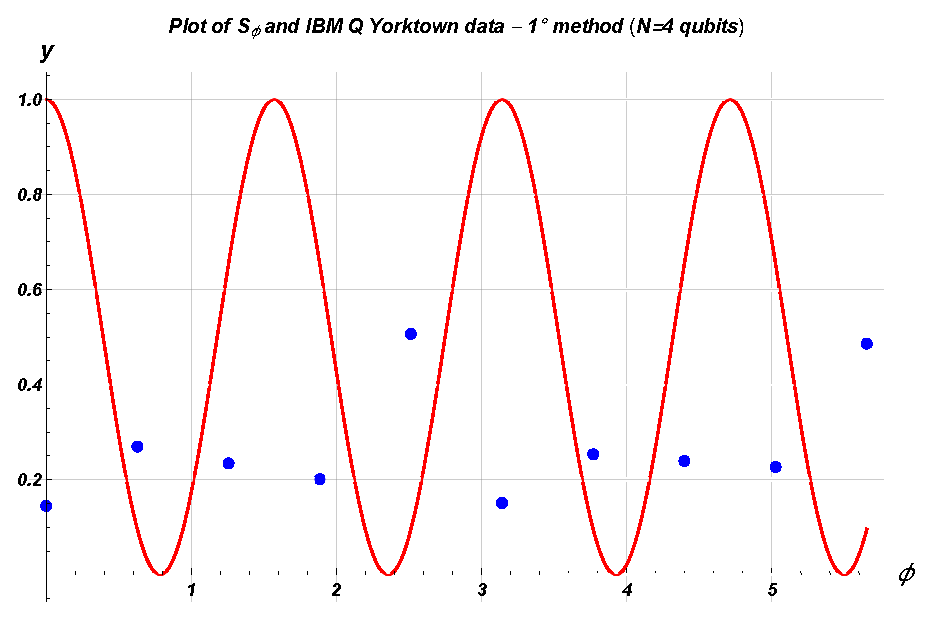
\includegraphics[width=1\textwidth]{./chapter3/graphics_IBM/real_device/S4.eps}
\end{minipage}
%\hspace{1mm}
\begin{minipage}[]{0.5\linewidth}
\centering 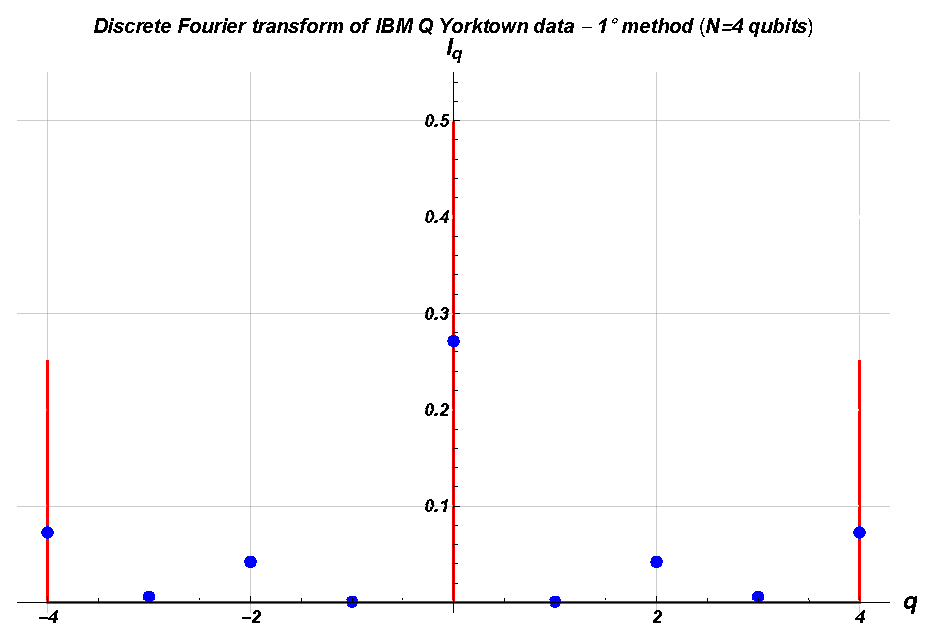
\includegraphics[width=1\textwidth]{./chapter3/graphics_IBM/real_device/I4.eps}
\end{minipage}
\caption{\label{RealDeviceIBMQX24} \textbf{N=4} qubits. Left:  plot of $S_{\phi}^{\text{ideal}}$ is represented in red, experimental measurements $S_{\phi}$ obtained by the simulation in the \textbf{IBM Q Yorktown} backend are drawn in blue. Right: corresponding MQC amplitudes $I_q$ of $S_\phi^{\text{ideal}}$ and $S_\phi$, respectively in red and blue.}
\end{figure}

\begin{figure}[h!]
\begin{minipage}[c]{0.5\linewidth}
\hspace{1cm}
\centering 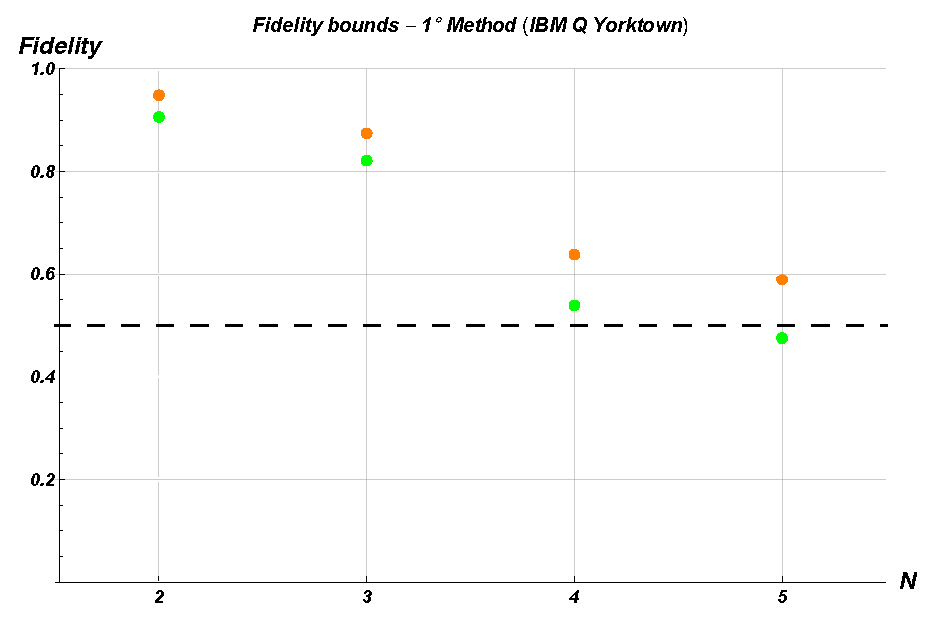
\includegraphics[width=1\textwidth]{./chapter3/graphics_IBM/real_device/F1Metodo.eps}
\end{minipage}
%\hspace{1mm}
\begin{minipage}[]{0.5\linewidth}
\centering 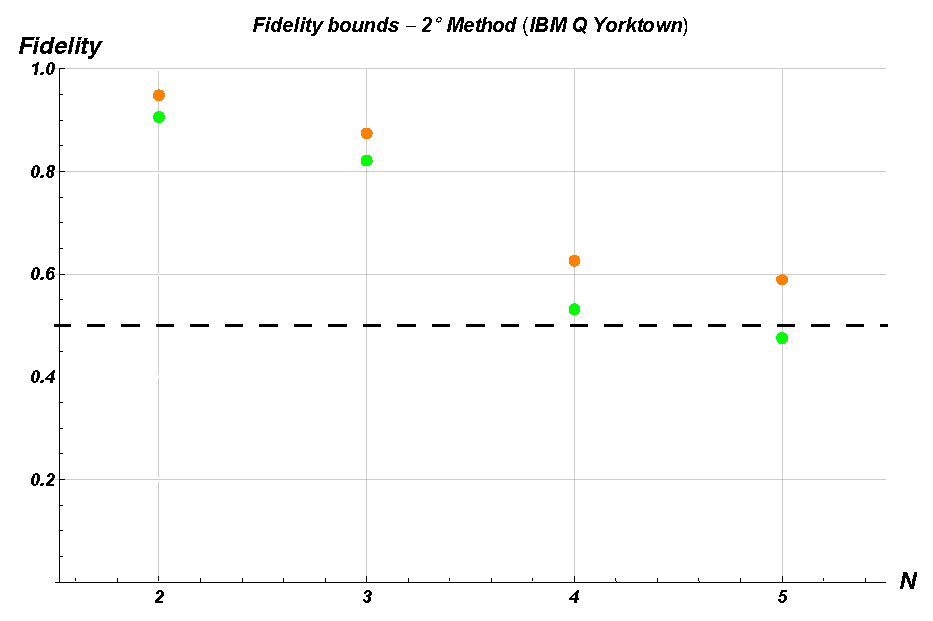
\includegraphics[width=1\textwidth]{./chapter3/graphics_IBM/real_device/F2Metodo.eps}
\end{minipage}
\caption{\label{Fidelity_RealDevice_ibmqx2} Fidelity lower bounds and upper bounds, respectively in green and orange, for the $N$-qubit MQC circuit, executed in the \textbf{IBM Q Yorktown} backend, are plotted in function of the number of qubits $N$. The line dashed in black represents the limit of 0.5 and under that we consider the fidelity of the state not acceptable. Left: first method plot. Right: second method plot.}
\end{figure}

\newpage

\subsubsection{Backend: IBM Q Melbourne}

Now, we consider the execution of the MQC circuit in the IBM Q Melbourne device, which supports 14 qubits.
 Its properties and coupling map are illustrated in Table \ref{ibmq_16_mealburne_parameters} and in Figure \ref{MelbourneLayout}. 
 We implement the circuit in both of the two ordering schemes, described above, for $N=1,\dots,6$ qubits.
 In the first method, the physical qubits used are $[0,1,\dots, 5]$ in order.
  In the second method, we distinguish two cases: for $N=2,3,4$, we do a better choice of the physical qubits used, while for $N=5,6$ we also slightly modify the circuit. 
 In Figure \ref{CircuitMQCModified_ibmqmelbourne}, we illustrate the new circuit implemented for $N=5$ qubits. The difference with the one in Figure \ref{MQCCircuit6} is that the CX gate is no more added between one qubit and its subsequent.

The results obtained by the two methods are quite different, unlike the IBM Q Yorktown device.
 The fidelity bounds in both cases are plotted in Figure \ref{Fidelity_RealDevice_ibmqmelbourne}.
  In the first case only the GHZ state for $N=2$ qubits is verified, in fact all the other fidelity bounds are not acceptable, because they are lower than 0.5.
   In the second case, the GHZ states for $N=2,3,4$ qubits are verified and the results for $N=5,6$ qubits are not acceptable, but they are however better than the first method. These surprisingly results show how the IBM Q Melbourne quantum device is highly sensitive to a correct qubits choice. It is also possible to notice that IBM Q Melbourne device is more unstable than the IBM Q Yorktown, due to the more number of qubits it has to manage. 
   To be thorough, in Figure \ref{RealDeviceIBMQMELBOURNE4} we show the $S_{\phi}$ and $I_q$ plots for $N=4$ qubits, obtained by the second method. 

\vspace{0.3cm}
\begin{figure}[h!]
\begin{equation*}
    \Qcircuit @C=1.2em @R=1.2em @!R {
	 	\lstick{\ket{0}_0} & \qw & \targ & \qw & \qw & \qw & \qw & \gate{U_{\phi}} 	& \qw & \qw 	& \qw 	& \qw 	& \targ 	& \qw 	& \qw & \meter \\
	 	\lstick{\ket{0}_1} & \gate{H} & \ctrl{-1} & \ctrl{1} & \qw & \qw & \qw & \gate{U_{\phi}} & \qw & \qw 	& \qw 	& \ctrl{1} 	& \ctrl{-1} & \gate{H}	& \qw & \meter \\
	 	\lstick{\ket{0}_2}& \qw & \qw & \targ & \ctrl{1} & \qw & \qw & \gate{U_{\phi}} 	& \qw& \qw 	& \ctrl{1} 	& \targ 	& \qw	 & \qw 	& \qw & \meter \\
	 	\lstick{\ket{0}_3} & \qw & \qw & \qw & \targ & \ctrl{1} & \qw & \gate{U_{\phi}}	 & \qw & \ctrl{1} & \targ 	& \qw 	& \qw	 & \qw 	& \qw & \meter \\
	 	\lstick{\ket{0}_4} & \qw & \qw & \qw & \qw & \targ & \qw & \gate{U_{\phi}} 		& \qw & \targ 	& \qw 	& \qw	 & \qw 	& \qw	 & \qw & \meter \\	 
	 }
\end{equation*}
\caption{\label{CircuitMQCModified_ibmqmelbourne} 5-qubit MQC circuit implemented in the IBM Q Melbourne device in the second method.}
\end{figure}

\vspace{0.3cm}

\begin{figure}[h!]
\begin{minipage}[c]{0.5\linewidth}
\hspace{1cm}
\centering 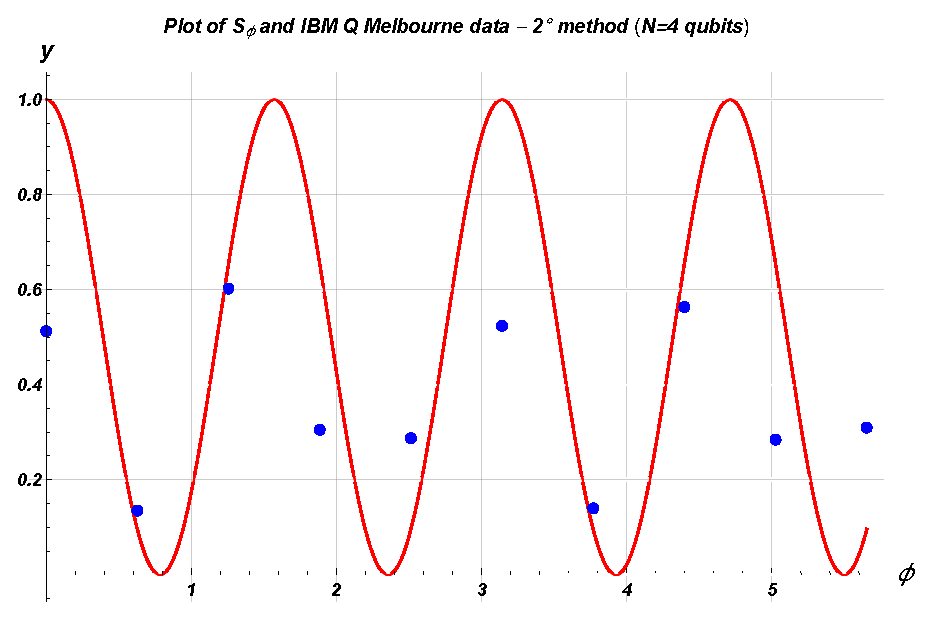
\includegraphics[width=1\textwidth]{./chapter3/graphics_IBM/real_device/S4_ibmqmelbourne.eps}
\end{minipage}
%\hspace{1mm}
\begin{minipage}[]{0.5\linewidth}
\centering 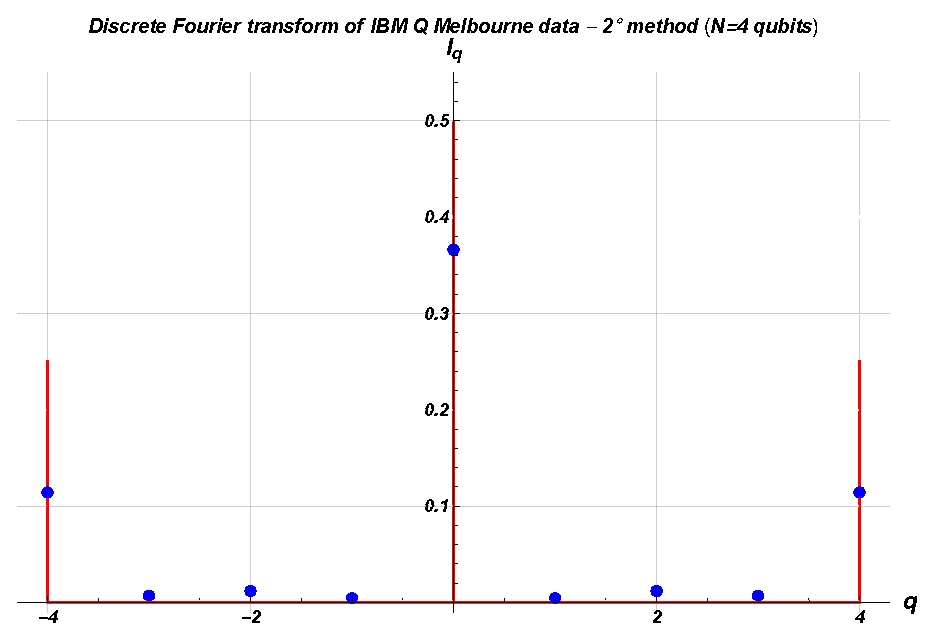
\includegraphics[width=1\textwidth]{./chapter3/graphics_IBM/real_device/I4_ibmqmelbourne.eps}
\end{minipage}
\caption{\label{RealDeviceIBMQMELBOURNE4} \textbf{N=4} qubits. Left:  plot of $S_{\phi}^{\text{ideal}}$ is represented in red, experimental measurements $S_{\phi}$ obtained by the simulation in the \textbf{IBM Q Melbourne} backend are drawn in blue. Right: corresponding MQC amplitudes $I_q$ of $S_\phi^{\text{ideal}}$ and $S_\phi$, respectively in red and blue.}
\end{figure}


\begin{figure}[h!]
\begin{minipage}[c]{0.5\linewidth}
\hspace{1cm}
\centering 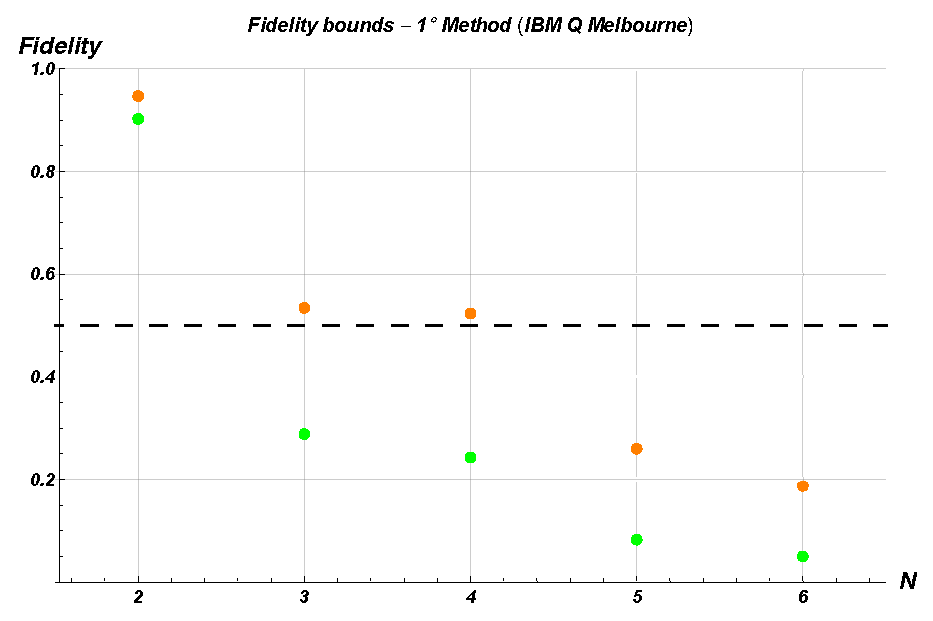
\includegraphics[width=1\textwidth]{./chapter3/graphics_IBM/real_device/F1Metodo_ibmqmelbourne.eps}
\end{minipage}
%\hspace{1mm}
\begin{minipage}[]{0.5\linewidth}
\centering 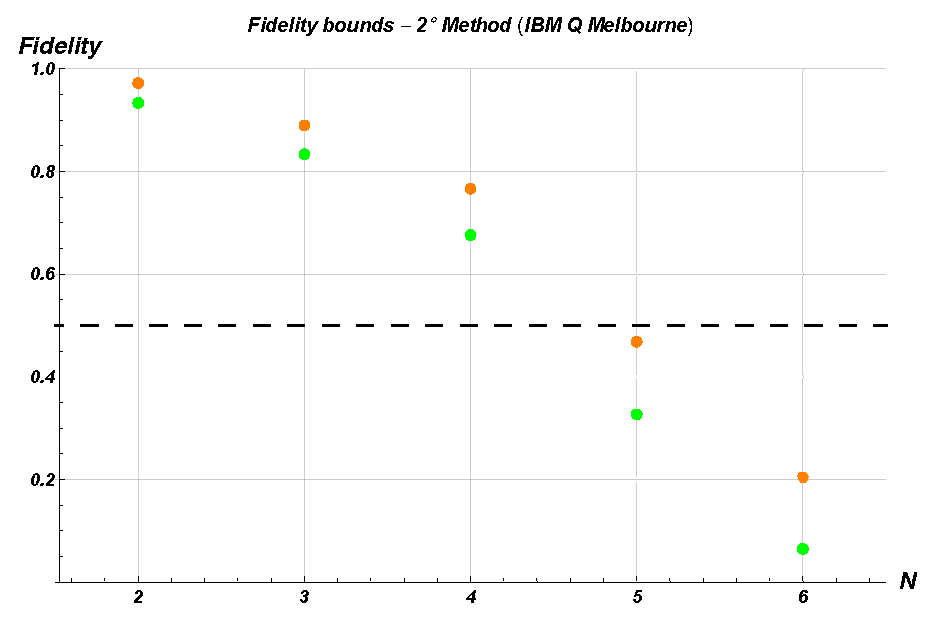
\includegraphics[width=1\textwidth]{./chapter3/graphics_IBM/real_device/F2Metodo_ibmqmelbourne.eps}
\end{minipage}
\caption{\label{Fidelity_RealDevice_ibmqmelbourne} Fidelity lower bounds and upper bounds, respectively in green and orange, for the $N$-qubit MQC circuit, executed in the \textbf{IBM Q Melbourne} backend, are plotted in function of the number of qubits $N$. The line dashed in black represents the limit of 0.5 and under that we consider the fidelity of the state not acceptable. Left: first method plot. Right: second method plot.}
\end{figure}





\begin{center}
\begin{table}[h!]
\begin{minipage}[c]{0.5\linewidth}
\hspace{1cm}
\[
\begin{array}{*{2}l}
\toprule
\text{N} 	&	\text{Physical qubits used}	 \\
\midrule
2	&	[0,1]  \\
3	&	[0,1,2] \\
4	&	[0,1,2,4]	 \\
5	&	[0,1,2,3,4]	\\
\bottomrule

\end{array}
\]
\end{minipage}
\begin{minipage}[]{0.5\linewidth}
\[
\begin{array}{*{2}l}
\toprule
\text{N} 	&	\text{Physical qubits used}	 \\
\midrule
2	&	[11,10] \\
3	&	[11,12,2] \\
4	&	[13,12,2,3]	 \\
5	&	[1,13,12,2,3]\\
6	&	[0,1,13,12,2,3]	\\
\bottomrule

\end{array}
\]

\end{minipage}


\caption{ Table of physical qubits used in the MQC circuit implemented in the real devices, in the second method. Left: IBM Q Yorktown device. Right: IBM Q Melbourne device. }
\label{physicalqubits}
\end{table}
\end{center}



\newpage
\section{MQC Circuit on Cirq software }
\label{Cirq_MqcCircuit}

Now, let us test the Cirq software, the Google quantum computer interface. The analysis is carried out in two phases.
First, we implement the MQC circuit for different values of $N$, in noiseless condition. The matrix  $U_{\phi}$ has the form of Eq. (\ref{U_gate_MQC}) and the results are obtained and analyzed as illustrated in the Section \ref{Qiskitsection}.
In particular, we execute the circuit for $N=2,\dots,22$ qubits on the Density Matrix Simulator with 6000 shots. The results $S_\phi$ and $I_q$ are the same of the ones obtained by the simulation in the Qasm Simulator of IBM in the ideal case, so they are not illustrated again. 
Then, we consider for instance the MQC circuit of $N=5$ qubits  \footnote{We note that with a computer of 8 Gb of RAM we could not simulate over than $N=12$ qubits in noisy condition, because of the high computational costs.} and we add different types of quantum channels on it; in fact, it is interesting to focus on a system with few qubits and answer to the question: how does the state change as a function of the parameters of the channels? 
We execute the circuit in the Density Matrix Simulator with 6000 shots and, for each type of channel, we plot the fidelity bounds as a function of the parameter of the channels.

\subsection{Adding quantum channels}
\label{protocol_insertion}

We add quantum noise channels to the MQC circuit illustrated in Section \ref{theory}. The main noise channels have been previously illustrated in Section \ref{QuantumChannels}. 
They are added to the circuit in the following way:

\begin{enumerate}
\item First, we choose the type of noise channel to add in the circuit. For instance, we consider the Amplitude damping channel or the Depolarizing channel.
\item The parameters of all the channels we will insert are fixed at the same value $\gamma$.
\item  Noise channels, all of the same type, are inserted to the circuit between any two contiguous unitary gates. In particular, we add the channel following a definite procedure: the number of channels inserted between one gate and its subsequent is proportional to the time interval between them. For instance, we divide in time slices the MQC circuit without any noise channels. Each slice represents a Moment of the circuit (see Section \ref{Cirq_section}). We suppose that the fixed time between two contiguous time slices is $\Delta t = 1\, \mu s$. Therefore, if for example two contiguous gate are four time slices distant, we insert four channels and each of them has the parameter fixed at the value $\gamma$. If they are one time slice distant, we insert only one channel.
\end{enumerate}

\vspace{0.2cm}

\noindent The new circuit is shown in Figure \ref{CircuitMQC_Noise}, where the noise channels are represented as single-qubit gates with a number $n$. The number value, of each gate symbol, represents the number of times the noise channel is inserted.

We execute the circuit for different values of the parameter of the channels in the Density Matrix Simulator with 6000 shots. In particular, the results for a fixed value are obtained and analyzed, as illustrated in Section \ref{analysis}. Then, we plot the fidelity bounds as a function of the fixed parameter of the channels. We take the larger value of the parameter acceptable, for which the fidelity bounds are upper than 0.5 and the 5-qubit GHZ state is verified. Afterwards, we calculate the maximum relaxation time associated to the channel. 
For example, suppose that the largest value of the parameter is $p$. The relaxation time $T$ is calculated from the relation:

\begin{equation}
p = 1 - e^{-\Delta t / T} \quad \Longrightarrow \quad T= -\frac{\Delta t}{\log{(1-p)}}.
 \label{RelaxationTimeFormula}
 \end{equation}

\noindent We underline that the values obtained are not reliable. In fact, more sophisticated experiments should be done for calculating the relaxation times of a system \cite{TutorialQiskit}. Therefore, they represent just an estimate and do not reflect the actual value.



\begin{figure}[h!]
\begin{equation*}
    \Qcircuit @C=0.4em @R=0.6em @!R {
	 	\lstick{\ket{0}_0} &  \gate{\text{\begin{tiny} 1 \end{tiny}}} &\gate{H} &\gate{\text{\begin{tiny} 1 \end{tiny}}} & \ctrl{1} &  \gate{\text{\begin{tiny} 4 \end{tiny}}} & \qw & \qw & \qw & \qw & \qw & \qw & 				\gate{U_{\phi}} 	& \qw & \qw 	& \qw 	& \qw 	\qw & \qw & \qw  &  \gate{\text{\begin{tiny} 4 \end{tiny}}} &  \ctrl{1} &\gate{\text{\begin{tiny} 1 \end{tiny}}}  & \gate{H} 	& \gate{\text{\begin{tiny} 1 \end{tiny}}} & \meter \\
	 	\lstick{\ket{0}_1} &   \gate{\text{\begin{tiny} 2 \end{tiny}}} & \qw & \qw & \targ &  \gate{\text{\begin{tiny} 1 \end{tiny}}} & \ctrl{1} &  \gate{\text{\begin{tiny} 3 \end{tiny}}} & \qw & \qw   &\qw & \qw & 			\gate{U_{\phi}} & \qw & \qw 	& \qw 	& \qw &  \gate{\text{\begin{tiny} 3 \end{tiny}}} & \ctrl{1} 	 &  \gate{\text{\begin{tiny} 1 \end{tiny}}} & \targ & \qw	& \qw & \gate{\text{\begin{tiny} 2 \end{tiny}}} &   \meter \\
	 	\lstick{\ket{0}_2}&  \gate{\text{\begin{tiny} 3 \end{tiny}}} & \qw & \qw &\qw & \qw &  \targ &  \gate{\text{\begin{tiny} 1 \end{tiny}}} & \ctrl{1} &  \gate{\text{\begin{tiny} 2 \end{tiny}}}  & \qw & \qw &			\gate{U_{\phi}} 	& \qw& \qw 	&  \gate{\text{\begin{tiny} 2 \end{tiny}}} & \ctrl{1} &  \gate{\text{\begin{tiny} 1 \end{tiny}}}	& \targ 	& \qw	 & \qw 	& \qw &  \qw & \gate{\text{\begin{tiny} 3 \end{tiny}}} &  \meter \\
	 	\lstick{\ket{0}_3} & \gate{\text{\begin{tiny} 4 \end{tiny}}}& \qw & \qw &\qw & \qw & \qw &\qw &  \targ & \gate{\text{\begin{tiny} 1 \end{tiny}}} & \ctrl{1} \qw &  \gate{\text{\begin{tiny} 1 \end{tiny}}} &	 	\gate{U_{\phi}}	 &  \gate{\text{\begin{tiny} 1 \end{tiny}}} & \ctrl{1} &  \gate{\text{\begin{tiny} 1 \end{tiny}}} & \targ 	& \qw 	& \qw	 & \qw 	& \qw &  \qw & \qw & \gate{\text{\begin{tiny} 4 \end{tiny}}} &  \meter \\
	 	\lstick{\ket{0}_4} & \gate{\text{\begin{tiny} 5 \end{tiny}}} & \qw & \qw & \qw & \qw & \qw & \qw & \qw & \qw& \targ &   \gate{\text{\begin{tiny} 1 \end{tiny}}} & 					\gate{U_{\phi}} 	 &  \gate{\text{\begin{tiny} 1 \end{tiny}}} & \targ 	& \qw 	& \qw	 & \qw 	& \qw	 & \qw & \qw &  \qw & \qw & \gate{\text{\begin{tiny} 5 \end{tiny}}} &  \meter \\	 
	 }
\end{equation*}
\caption{\label{CircuitMQC_Noise} $5$-qubit MQC circuit  with quantum noise channels. The number value, of each gate symbol, represents the number of times the noise channel is inserted.}
\end{figure}

\noindent Now, we apply the procedure described in the case we add  respectively  only Amplitude Damping or Depolarizing channels.

\subsubsection{Amplitude damping channels}

In Figure \ref{AmplitudeDamping_metodo}, we illustrate the fidelity bounds of the 5-qubit GHZ state as a function of the parameter $\gamma$ of the Amplitude Damping channel. The state is verified until the parameter reaches the value of $p=0.08$. The relaxation time is calculated as in Eq. (\ref{RelaxationTimeFormula}) and it results $T_{AD}=11.99\, \mu s$. We remind that, for the Amplitude Damping channel, the relaxation time $T_{AD}$ is the time in which the state of the system decays into the ground state  (see Section \ref{Amp_section}). Therefore, if we suppose that $\Delta t = 1\, \mu s$ is the time between the application of two subsequent gates, after $\sim 12$ gate applications, the state decays into the ground state.

\begin{figure}[h!]
\centering 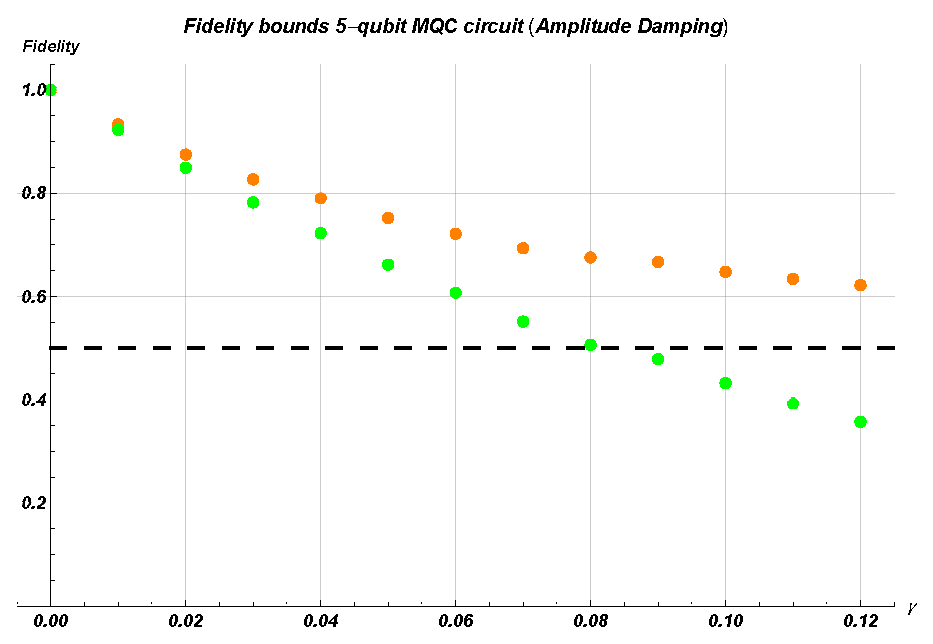
\includegraphics[width=0.7\textwidth]{./chapter3/Cirq_nuovo/Amp_gamma.eps}
\caption{\label{AmplitudeDamping_metodo} Fidelity lower bounds and upper bounds, respectively in green and orange, for the $5$-qubit MQC circuit, executed in the Density Matrix Simulator, are plotted in function of the values of the \textbf{Amplitude Damping} channel parameter. The line dashed in black represents the limit of 0.5 and under that we consider the fidelity of the state not acceptable.}
\end{figure}


\subsubsection{Depolarizing channels}

In Figure \ref{Depolarizing_metodo}, we illustrate the fidelity bounds of the 5-qubit GHZ state as a function of the parameter $\gamma$ of the Depolarizing channel. The state is verified until the parameter reaches the value of $p=0.022$. The relaxation time is calculated as in Eq. (\ref{RelaxationTimeFormula}) and it results $T_D=44.95\, \mu s$. For the Depolarizing channel, the relaxation time $T_D$ is the time in which the state of the system decays into a completely mixed state (see Section \ref{Dep_section}).
Therefore, it decays after $\sim45$ gate operations.

\begin{figure}[h!]
\centering 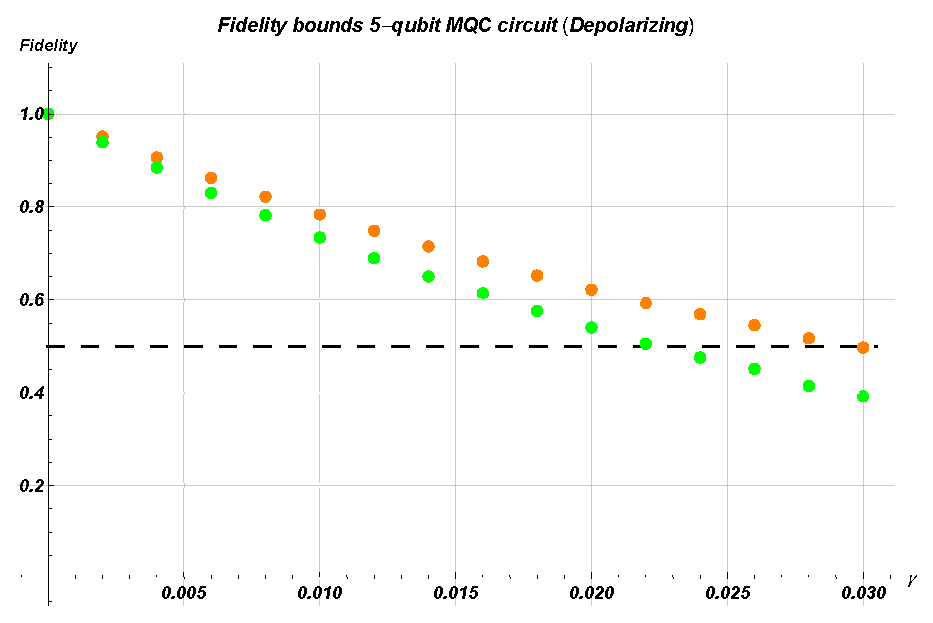
\includegraphics[width=0.7\textwidth]{./chapter3/Cirq_nuovo/Dep_p.eps}
\caption{\label{Depolarizing_metodo} Fidelity lower bounds and upper bounds, respectively in green and orange, for the $5$-qubit MQC circuit, executed in the Density Matrix Simulator, are plotted in function of the values of the \textbf{Depolarizing} channel parameter. The line dashed in black represents the limit of 0.5 and under that we consider the fidelity of the state not acceptable.
}
\end{figure}

In conclusion, we note that $T_{AD} < T_{D}$, therefore the largest time for which the state does not decay is $T_{AD}$. In reality, the effects act together, so probably even less time would be obtained.

\section{GHZ state: density matrix elements}

Another way to recognize a GHZ state is to study some peculiar matrix elements, i.e. the four corners of the density matrix of the system. In fact, for an ideal GHZ state, the nonzero elements in the density matrix reside only in the four corners and their value is of 0.5. Therefore, we consider a 5-qubit GHZ state prepared following the protocol illustrated in Section \ref{protocol_insertion} and the circuit implementation is shown in Figure \ref{Circuit_DensityMatrix}. As done previously, we distinguish two cases with noise due only to Amplitude Damping channels or only to Depolarizing channels.  We fix the parameter $\gamma$ of the channels and we simulate the circuit in the Density Matrix Simulator. Then, we analyze the goodness of the state obtained by measuring the four corners of the density matrix of the system. 

\begin{figure}[h!]
\begin{equation*}
    \Qcircuit @C=0.4em @R=0.6em @!R {
	 	\lstick{\ket{0}_0} &  \gate{\text{\begin{tiny} 1 \end{tiny}}} & \gate{H} &  \gate{\text{\begin{tiny} 1 \end{tiny}}} & \ctrl{1} &  \gate{\text{\begin{tiny} 4 \end{tiny}}} & \qw & \qw & \qw & \qw & \qw & \qw  		& \qw 	 \\
	 	\lstick{\ket{0}_1} &  \gate{\text{\begin{tiny} 2 \end{tiny}}} &  \qw & \qw & \targ &  \gate{\text{\begin{tiny} 1 \end{tiny}}} & \ctrl{1} &  \gate{\text{\begin{tiny} 3 \end{tiny}}} & \qw & \qw   &\qw & \qw  	& \qw 	 \\
	 	\lstick{\ket{0}_2}&  \gate{\text{\begin{tiny} 3 \end{tiny}}} &  \qw &  \qw &\qw & \qw &  \targ &  \gate{\text{\begin{tiny} 1 \end{tiny}}} & \ctrl{1} &  \gate{\text{\begin{tiny} 2 \end{tiny}}}  & \qw & \qw & \qw  \\
	 	\lstick{\ket{0}_3} &  \gate{\text{\begin{tiny} 4 \end{tiny}}} &  \qw &  \qw &\qw & \qw & \qw &\qw &  \targ & \gate{\text{\begin{tiny} 1 \end{tiny}}} & \ctrl{1} \qw &  \gate{\text{\begin{tiny} 1 \end{tiny}}} & \qw  \\
	 	\lstick{\ket{0}_4} & \gate{\text{\begin{tiny} 5 \end{tiny}}} &  \qw & \qw & \qw & \qw & \qw & \qw & \qw & \qw& \targ &   \gate{\text{\begin{tiny} 1 \end{tiny}}} & \qw \\	 
	 }
\end{equation*}
\caption{\label{Circuit_DensityMatrix} $5$-qubit circuit with quantum noise channels. The number value, of each gate symbol, represents the number of times the noise channel is inserted.}
\end{figure}


%as a function of the parameters of the channels.

\subsubsection{Amplitude damping channels}

In Figure \ref{AmplitudeDamping_matrici}, we show the value of the four corners elements of the density matrix of the system as a function of the parameter $\gamma$ of the Amplitude Damping channel. We note that by increasing the parameter value, the system state decays into the ground state: the matrix element $\rho_{00}$ tends asymptotically to 1, while the other tend to 0.



\begin{figure}[h!]
\begin{minipage}[c]{0.5\linewidth}
\hspace{1cm}
\centering 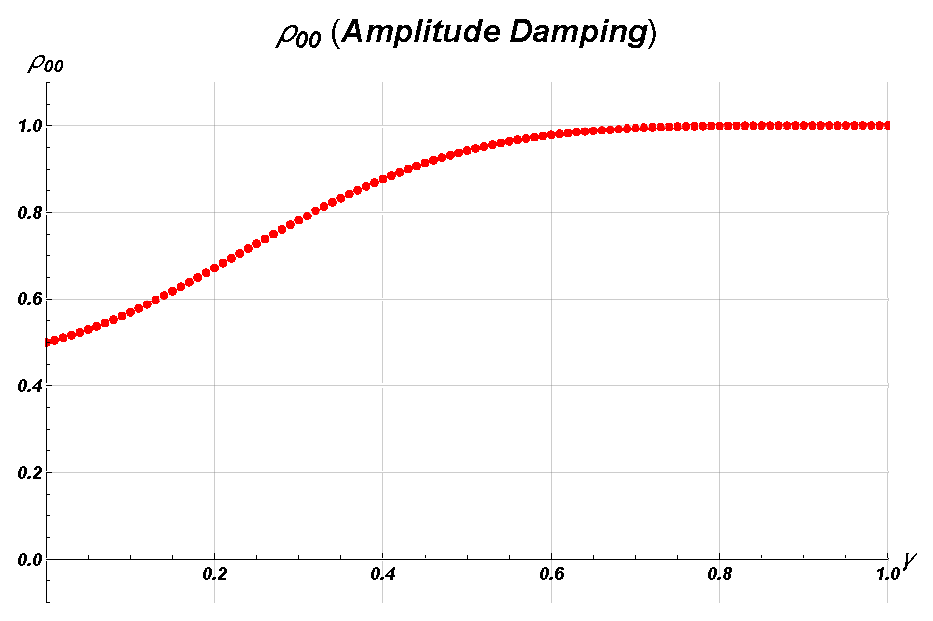
\includegraphics[width=0.78\textwidth]{./chapter3/Cirq_nuovo/decoerenza/amp_00.eps}
\end{minipage}
%\hspace{1mm}
\begin{minipage}[]{0.5\linewidth}
\centering 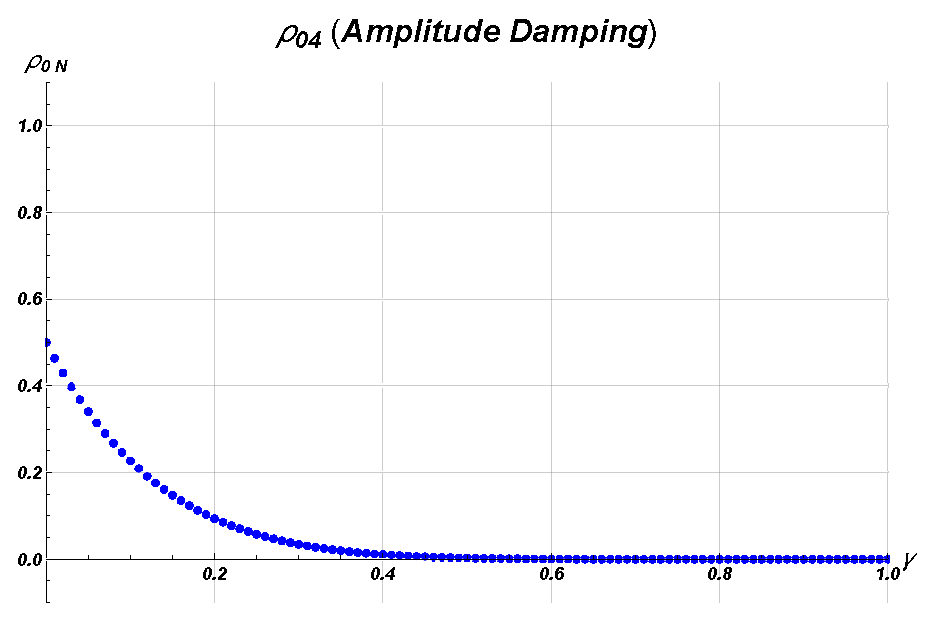
\includegraphics[width=0.78\textwidth]{./chapter3/Cirq_nuovo/decoerenza/amp_0N.eps}
\end{minipage} \\
\begin{minipage}[c]{0.5\linewidth}
\hspace{1cm}
\centering 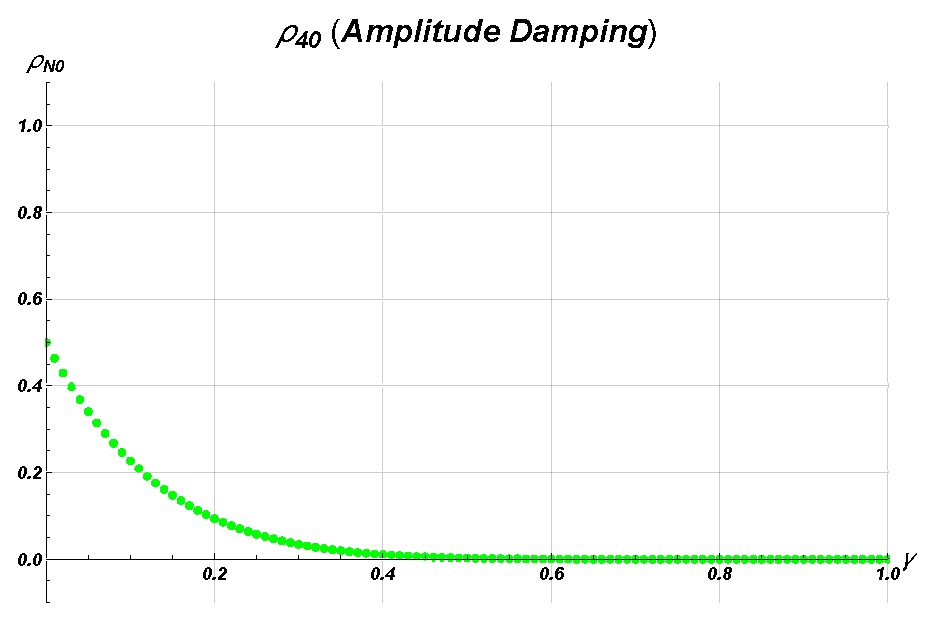
\includegraphics[width=0.78\textwidth]{./chapter3/Cirq_nuovo/decoerenza/amp_N0.eps}
\end{minipage}
%\hspace{1mm}
\begin{minipage}[]{0.5\linewidth}
\centering 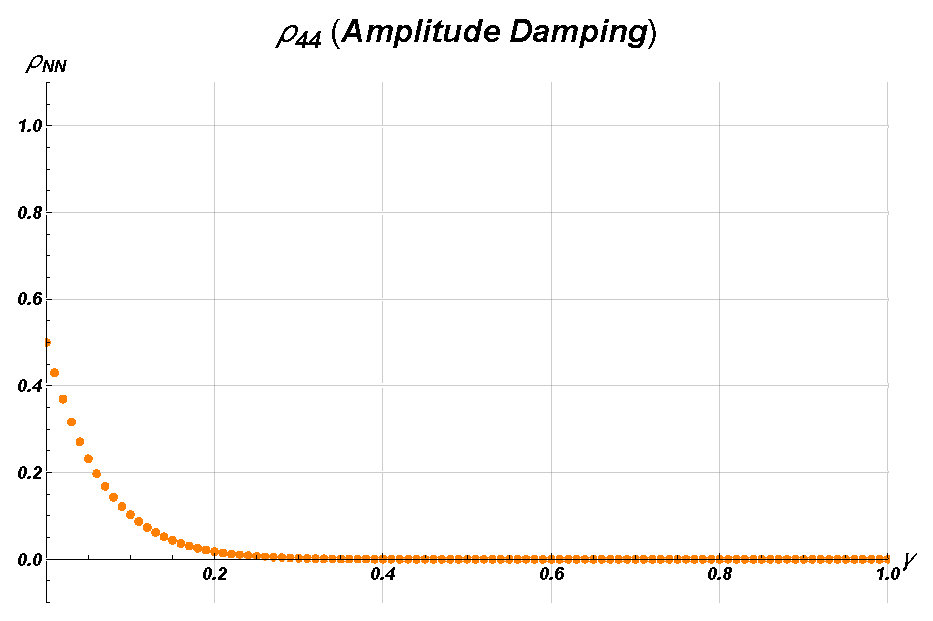
\includegraphics[width=0.78\textwidth]{./chapter3/Cirq_nuovo/decoerenza/amp_NN.eps}
\end{minipage}
\caption{\label{AmplitudeDamping_matrici} Corner elements of the density matrix of the 5-qubit system in function of the parameter $\gamma$ of the \textbf{Amplitude Damping} channel. The system state decays into the ground state.}
\end{figure}

\vspace{-0.4cm}
\subsubsection{Depolarizing channels}
In Figure \ref{Depolarizing_matrici}, we show the value of the four corners elements of the density matrix of the system as a function of the parameter $\gamma$ of the Depolarizing channel. 

\begin{figure}[h!]
\begin{minipage}[c]{0.5\linewidth}
\hspace{1cm}
\centering 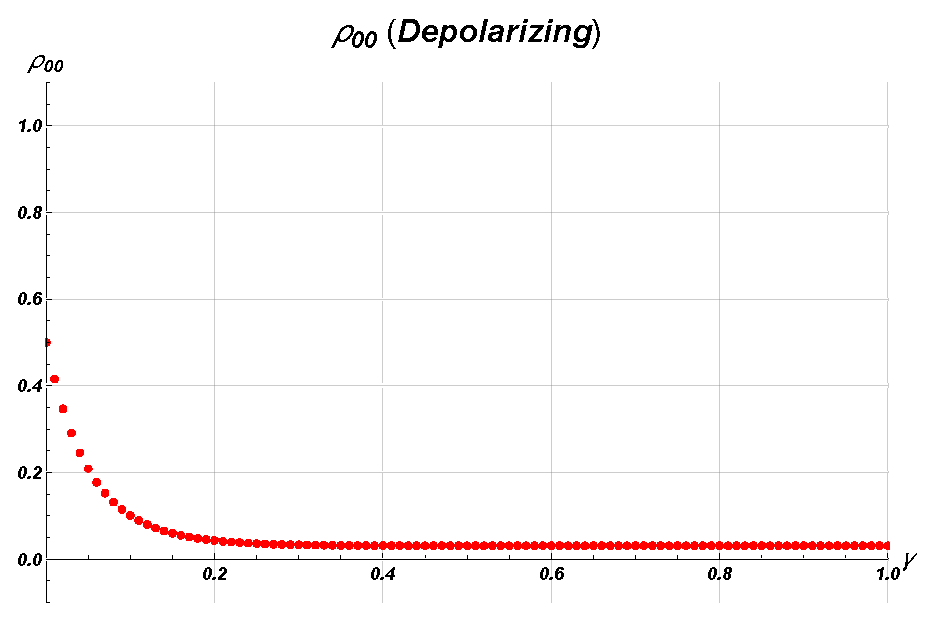
\includegraphics[width=0.78\textwidth]{./chapter3/Cirq_nuovo/decoerenza/dep_00.eps}
\end{minipage}
%\hspace{1mm}
\begin{minipage}[]{0.5\linewidth}
\centering 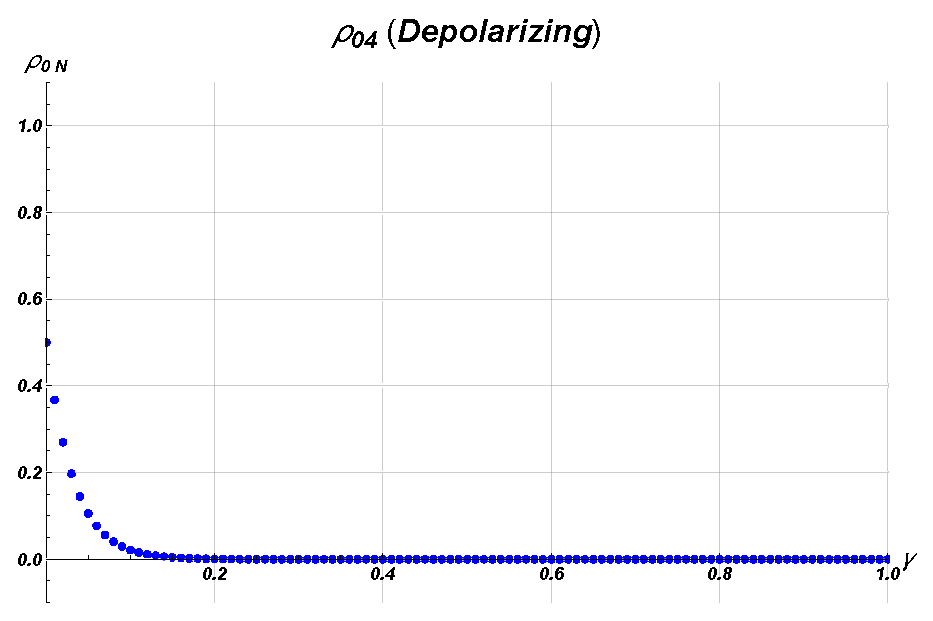
\includegraphics[width=0.78\textwidth]{./chapter3/Cirq_nuovo/decoerenza/dep_0N.eps}
\end{minipage} \\
\begin{minipage}[c]{0.5\linewidth}
\hspace{1cm}
\centering 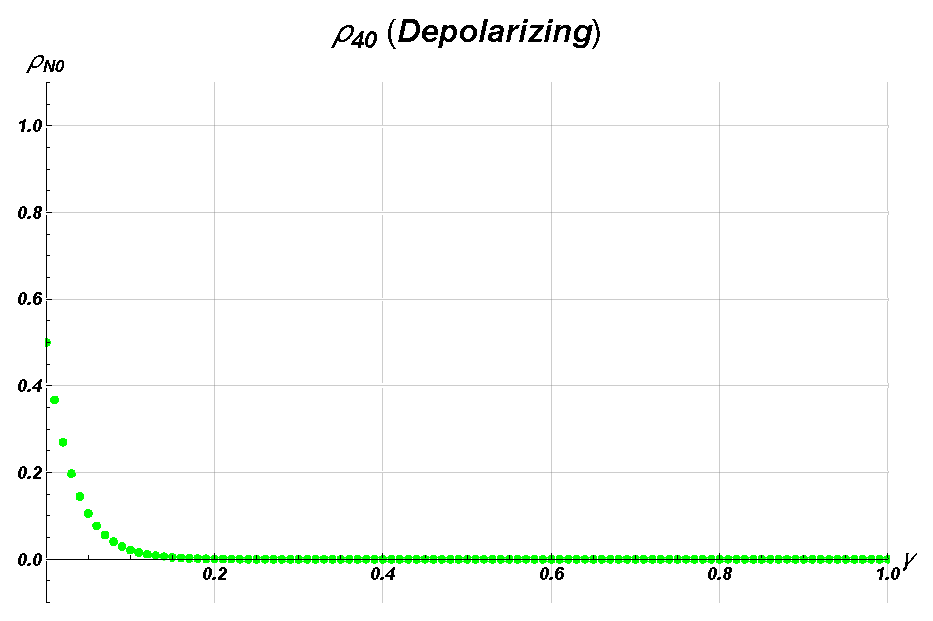
\includegraphics[width=0.78\textwidth]{./chapter3/Cirq_nuovo/decoerenza/dep_N0.eps}
\end{minipage}
%\hspace{1mm}
\begin{minipage}[]{0.5\linewidth}
\centering 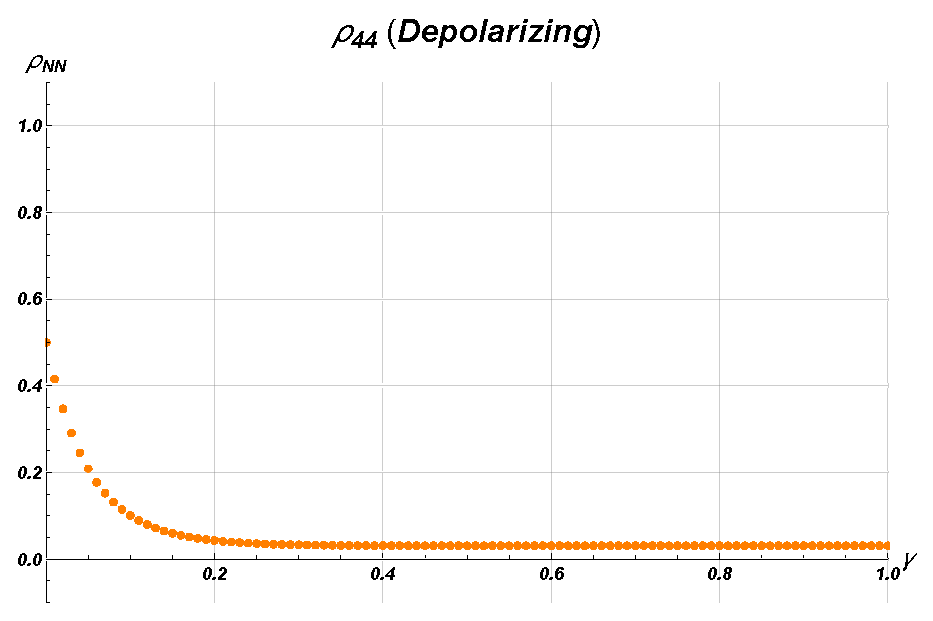
\includegraphics[width=0.78\textwidth]{./chapter3/Cirq_nuovo/decoerenza/dep_NN.eps}
\end{minipage}
\caption{\label{Depolarizing_matrici} Corner elements of the density matrix of the 5-qubit system in function of the parameter $\gamma$ of the \textbf{Depolarizing} channel. The system state decays into a completely mixed state.}
\end{figure}

\noindent For the Depolarizing channel, we note that by increasing the parameter value, the system state decays into a completely mixed state, for which the nonzero density matrix elements have the same value and reside only in the diagonal. In particular, the density matrix of the 5-qubit system we are considering, has the form $32\times32$, therefore the elements $\rho_{00}$ and $\rho_{44}$ tend to $\frac{1}{32}$, as we can see in Figure \ref{Depolarizing_matrici}. Also the other elements in the diagonal tend to this value, while all the elements outside tend to 0.



\section{Bell state: concurrence measurements}

In the Cirq software, we implement a simple circuit of $N=2$ qubits that makes a \textit{Bell state}. Quantum channels are added following the protocol illustrated in Section \ref{protocol_insertion}. Firstly, we insert only Amplitude Damping channels in the circuit, then only Depolarizing channels.
The circuit for both configuration is illustrated in Figure \ref{Circuit_piccolo}.


\begin{figure}[h!]
\begin{equation*}
    \Qcircuit @C=1.2em @R=0.9em @!R {
	 	\lstick{\ket{0}_0} &  \gate{\text{\begin{tiny} 1 \end{tiny}}} & \gate{H} & \gate{\text{\begin{tiny} 1 \end{tiny}}} &  \ctrl{1} &  \gate{\text{\begin{tiny} 1 \end{tiny}}} & \qw  \\
	 	\lstick{\ket{0}_1} &   \gate{\text{\begin{tiny} 2 \end{tiny}}} & \qw & \qw & \targ &  \gate{\text{\begin{tiny} 1 \end{tiny}}}  	& \qw 	 \\
	 }
\end{equation*}
\caption{\label{Circuit_piccolo}  $2$-qubit circuit with quantum noise channels. The number value, of each gate symbol, represents the number of times the noise channel is inserted.}
\end{figure}

\noindent For both configuration, we fix the parameter $\gamma$ of the channels and we simulate the circuit in the Density Matrix Simulator, that gives us the access to the density matrix of the state. 
We quantify the order of entanglement of the state by doing \textbf{concurrence} measurements, defined in Eq. (\ref{18_2_firstchapter}). For each case, the concurrence values are plotted as a function of the parameter of the channels in Figure \ref{Concurrence_entrambi}. As we expected, the concurrence value decreases when the parameter value increases.

\vspace{0.3cm}

\begin{figure}[h!]
\begin{minipage}[c]{0.5\linewidth}
\hspace{1cm}
\centering 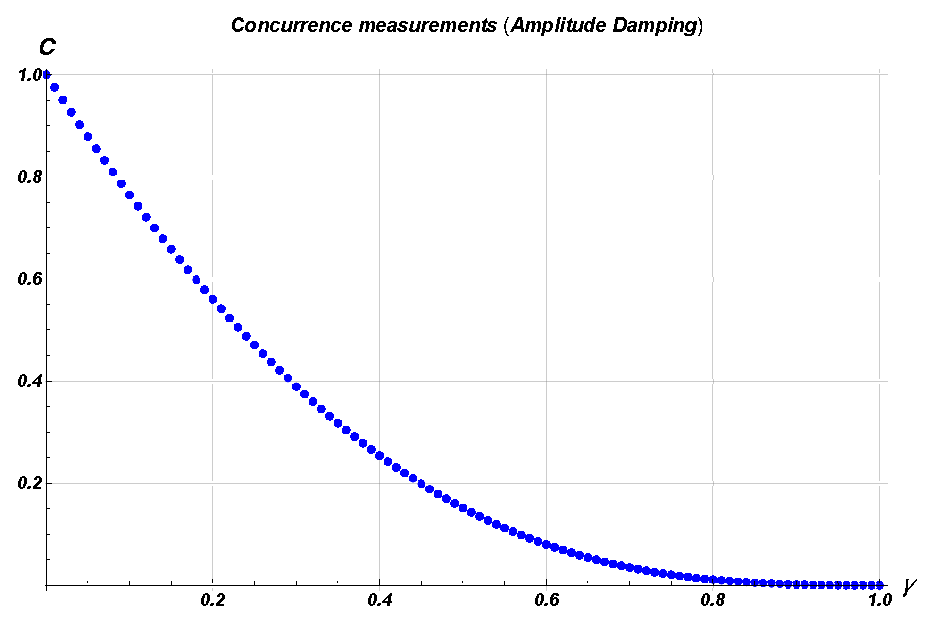
\includegraphics[width=1\textwidth]{./chapter3/Cirq_nuovo/concurrence/Concurrence_Amplitude.eps}
\end{minipage}
%\hspace{1mm}
\begin{minipage}[]{0.5\linewidth}
\centering 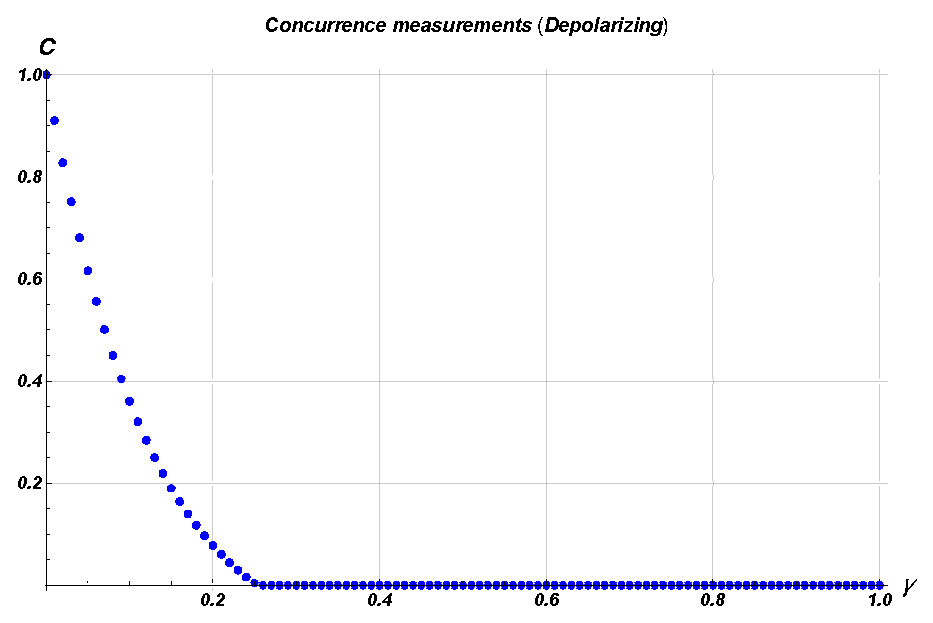
\includegraphics[width=1\textwidth]{./chapter3/Cirq_nuovo/concurrence/Concurrence_Depolarizing.eps}
\end{minipage}
\caption{\label{Concurrence_entrambi} Concurrence values for the 2-qubit system as a function of the parameter $\gamma$ of the channels. Top: only Amplitude Damping channels are inserted into the circuit. Bottom: only Depolarizing channels are inserted into the circuit. }
\end{figure}




%\begin{figure}[h!]
%\begin{minipage}[c]{0.5\linewidth}
%\hspace{1cm}
%\centering \includegraphics[width=0.95\textwidth]{./chapter3/Cirq_nuovo/concurrence/4plot.eps}
%\end{minipage}
%%\hspace{1mm}
%\begin{minipage}[]{0.5\linewidth}
%\centering 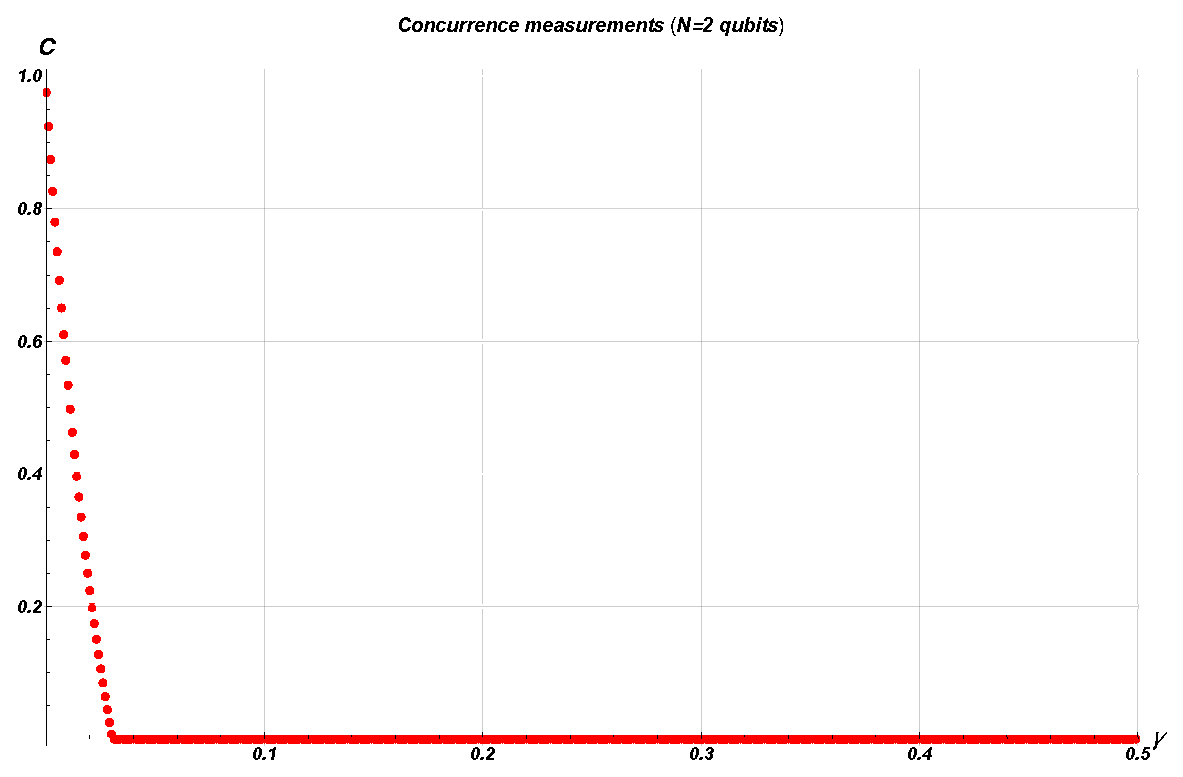
\includegraphics[width=0.95\textwidth]{./chapter3/Cirq_nuovo/concurrence/5plot.eps}
%\end{minipage} 
%\caption{\label{AmplitudeDamping_metodo} 
%%Fidelity lower bounds and upper bounds, respectively in blue and red. Amplitude damping channels are added in the MQC circuit of $N=5$ qubits as in Figure \ref{CircuitMQC_Amplitudedamping_1}. The circuit is executed on 'DensityMatrix' simulator for 1000 shots. Left: plot in the first case. Right: plot in the second case. The line dashed in black represents the limit of 0.5 and under that we consider the fidelity not acceptable.
%}
%\end{figure}


